% Options for packages loaded elsewhere
% Options for packages loaded elsewhere
\PassOptionsToPackage{unicode}{hyperref}
\PassOptionsToPackage{hyphens}{url}
%
\documentclass[
  ignorenonframetext,
  aspectratio=169,
]{beamer}
\newif\ifbibliography
\usepackage{pgfpages}
\setbeamertemplate{caption}[numbered]
\setbeamertemplate{caption label separator}{: }
\setbeamercolor{caption name}{fg=normal text.fg}
\beamertemplatenavigationsymbolsempty
% remove section numbering
\setbeamertemplate{part page}{
  \centering
  \begin{beamercolorbox}[sep=16pt,center]{part title}
    \usebeamerfont{part title}\insertpart\par
  \end{beamercolorbox}
}
\setbeamertemplate{section page}{
  \centering
  \begin{beamercolorbox}[sep=12pt,center]{section title}
    \usebeamerfont{section title}\insertsection\par
  \end{beamercolorbox}
}
\setbeamertemplate{subsection page}{
  \centering
  \begin{beamercolorbox}[sep=8pt,center]{subsection title}
    \usebeamerfont{subsection title}\insertsubsection\par
  \end{beamercolorbox}
}
% Prevent slide breaks in the middle of a paragraph
\widowpenalties 1 10000
\raggedbottom
\AtBeginPart{
  \frame{\partpage}
}
\AtBeginSection{
  \ifbibliography
  \else
    \frame{\sectionpage}
  \fi
}
\AtBeginSubsection{
  \frame{\subsectionpage}
}
\usepackage{iftex}
\ifPDFTeX
  \usepackage[T1]{fontenc}
  \usepackage[utf8]{inputenc}
  \usepackage{textcomp} % provide euro and other symbols
\else % if luatex or xetex
  \usepackage{unicode-math} % this also loads fontspec
  \defaultfontfeatures{Scale=MatchLowercase}
  \defaultfontfeatures[\rmfamily]{Ligatures=TeX,Scale=1}
\fi
\usepackage{lmodern}

\usetheme[]{Berlin}
\ifPDFTeX\else
  % xetex/luatex font selection
\fi
% Use upquote if available, for straight quotes in verbatim environments
\IfFileExists{upquote.sty}{\usepackage{upquote}}{}
\IfFileExists{microtype.sty}{% use microtype if available
  \usepackage[]{microtype}
  \UseMicrotypeSet[protrusion]{basicmath} % disable protrusion for tt fonts
}{}
\makeatletter
\@ifundefined{KOMAClassName}{% if non-KOMA class
  \IfFileExists{parskip.sty}{%
    \usepackage{parskip}
  }{% else
    \setlength{\parindent}{0pt}
    \setlength{\parskip}{6pt plus 2pt minus 1pt}}
}{% if KOMA class
  \KOMAoptions{parskip=half}}
\makeatother


\usepackage{longtable,booktabs,array}
\usepackage{calc} % for calculating minipage widths
\usepackage{caption}
% Make caption package work with longtable
\makeatletter
\def\fnum@table{\tablename~\thetable}
\makeatother
\usepackage{graphicx}
\makeatletter
\newsavebox\pandoc@box
\newcommand*\pandocbounded[1]{% scales image to fit in text height/width
  \sbox\pandoc@box{#1}%
  \Gscale@div\@tempa{\textheight}{\dimexpr\ht\pandoc@box+\dp\pandoc@box\relax}%
  \Gscale@div\@tempb{\linewidth}{\wd\pandoc@box}%
  \ifdim\@tempb\p@<\@tempa\p@\let\@tempa\@tempb\fi% select the smaller of both
  \ifdim\@tempa\p@<\p@\scalebox{\@tempa}{\usebox\pandoc@box}%
  \else\usebox{\pandoc@box}%
  \fi%
}
% Set default figure placement to htbp
\def\fps@figure{htbp}
\makeatother


% definitions for citeproc citations
\NewDocumentCommand\citeproctext{}{}
\NewDocumentCommand\citeproc{mm}{%
  \begingroup\def\citeproctext{#2}\cite{#1}\endgroup}
\makeatletter
 % allow citations to break across lines
 \let\@cite@ofmt\@firstofone
 % avoid brackets around text for \cite:
 \def\@biblabel#1{}
 \def\@cite#1#2{{#1\if@tempswa , #2\fi}}
\makeatother
\newlength{\cslhangindent}
\setlength{\cslhangindent}{1.5em}
\newlength{\csllabelwidth}
\setlength{\csllabelwidth}{3em}
\newenvironment{CSLReferences}[2] % #1 hanging-indent, #2 entry-spacing
 {\begin{list}{}{%
  \setlength{\itemindent}{0pt}
  \setlength{\leftmargin}{0pt}
  \setlength{\parsep}{0pt}
  % turn on hanging indent if param 1 is 1
  \ifodd #1
   \setlength{\leftmargin}{\cslhangindent}
   \setlength{\itemindent}{-1\cslhangindent}
  \fi
  % set entry spacing
  \setlength{\itemsep}{#2\baselineskip}}}
 {\end{list}}
\usepackage{calc}
\newcommand{\CSLBlock}[1]{\hfill\break\parbox[t]{\linewidth}{\strut\ignorespaces#1\strut}}
\newcommand{\CSLLeftMargin}[1]{\parbox[t]{\csllabelwidth}{\strut#1\strut}}
\newcommand{\CSLRightInline}[1]{\parbox[t]{\linewidth - \csllabelwidth}{\strut#1\strut}}
\newcommand{\CSLIndent}[1]{\hspace{\cslhangindent}#1}



\setlength{\emergencystretch}{3em} % prevent overfull lines

\providecommand{\tightlist}{%
  \setlength{\itemsep}{0pt}\setlength{\parskip}{0pt}}



 


\usepackage{tikz}
\usetikzlibrary{calc,positioning}
\usepackage{booktabs}
\usepackage{array}
\usepackage{xcolor}
\usepackage{amsmath}
\usepackage{amssymb}
\usepackage{physics}
\usepackage{verbatim}
\usepackage{adjustbox}
\usepackage{multirow}
\usepackage{caption}

% Custom colors
\definecolor{ColorUFV2}{RGB}{80,115,0}
\definecolor{ColorUFV}{RGB}{170,185,100}
\definecolor{mygray}{rgb}{0.6,0.6,0.6}

% Progress bar with frame numbers
\newcommand{\progressbar}{%
\pgfmathsetmacro{\theta}{360/\inserttotalframenumber*\insertframenumber}
\begin{tikzpicture}[scale=0.035]
\fill[ColorUFV] (0,0) circle (9);
\fill[ColorUFV2] (0,0) -- (9,0) arc (0:-\theta:9) -- cycle;
\fill[white] (0,0) circle (5);
\node at (0,0) {\tiny \insertframenumber};
\end{tikzpicture}
}

% Footline with progress bar and frame numbers
\setbeamertemplate{footline}{%
  \hfill%
 % \progressbar%
 \insertframenumber / \inserttotalframenumber
  }

% Remove navigation symbols
\setbeamertemplate{navigation symbols}{}

% Color settings
\setbeamercolor*{structure}{bg=ColorUFV,fg=ColorUFV2}
\setbeamertemplate{caption}[numbered]
\setbeamercolor*{palette primary}{use=structure,fg=white,bg=structure.fg}
\setbeamercolor*{palette secondary}{use=ColorUFV, fg=white, bg=ColorUFV}
\setbeamercolor*{palette tertiary}{use=structure,fg=white,bg=black}
\setbeamercolor*{palette quaternary}{fg=white,bg=black}
\setbeamercolor{section in toc}{fg=black,bg=white}
\setbeamercolor{alerted text}{use=structure,fg=structure.fg!50!black!80!black}
\setbeamercolor{titlelike}{parent=ColorUFV,fg=white, bg=ColorUFV2}
\setbeamercolor{frametitle}{bg=white,fg=ColorUFV2}
\setbeamercolor{block title}{fg=black,bg=black!10}
\setbeamercolor{block body}{fg=white,bg=ColorUFV2}

\setbeamercovered{transparent}
\useinnertheme{rounded}
\logo{
\includegraphics[height=0.5cm]{misc/logo-Esalq.png}}
\makeatletter
\@ifpackageloaded{caption}{}{\usepackage{caption}}
\AtBeginDocument{%
\ifdefined\contentsname
  \renewcommand*\contentsname{Table of contents}
\else
  \newcommand\contentsname{Table of contents}
\fi
\ifdefined\listfigurename
  \renewcommand*\listfigurename{List of Figures}
\else
  \newcommand\listfigurename{List of Figures}
\fi
\ifdefined\listtablename
  \renewcommand*\listtablename{List of Tables}
\else
  \newcommand\listtablename{List of Tables}
\fi
\ifdefined\figurename
  \renewcommand*\figurename{Figure}
\else
  \newcommand\figurename{Figure}
\fi
\ifdefined\tablename
  \renewcommand*\tablename{Table}
\else
  \newcommand\tablename{Table}
\fi
}
\@ifpackageloaded{float}{}{\usepackage{float}}
\floatstyle{ruled}
\@ifundefined{c@chapter}{\newfloat{codelisting}{h}{lop}}{\newfloat{codelisting}{h}{lop}[chapter]}
\floatname{codelisting}{Listing}
\newcommand*\listoflistings{\listof{codelisting}{List of Listings}}
\makeatother
\makeatletter
\makeatother
\makeatletter
\@ifpackageloaded{caption}{}{\usepackage{caption}}
\@ifpackageloaded{subcaption}{}{\usepackage{subcaption}}
\makeatother

\usepackage{bookmark}
\IfFileExists{xurl.sty}{\usepackage{xurl}}{} % add URL line breaks if available
\urlstyle{same}
\hypersetup{
  pdftitle={Selection indexes in plant breeding},
  pdfauthor={José Tiago Barroso Chagas},
  hidelinks,
  pdfcreator={LaTeX via pandoc}}


\title{Selection indexes in plant breeding}
\subtitle{Métodos de melhoramento LGN-5801}
\author{José Tiago Barroso Chagas}
\date{2025-11-19}
\institute{Escola Superior de Agricultura Luiz de Queiroz - Universidade
de São Paulo}

\begin{document}
\frame{\titlepage}

\renewcommand*\contentsname{Outline}
\begin{frame}[allowframebreaks]
  \frametitle{Outline}
  \setcounter{tocdepth}{3}
  \tableofcontents
\end{frame}
\setcounter{tocdepth}{3}
\tableofcontents
}

\begin{frame}{Background}
\phantomsection\label{background}
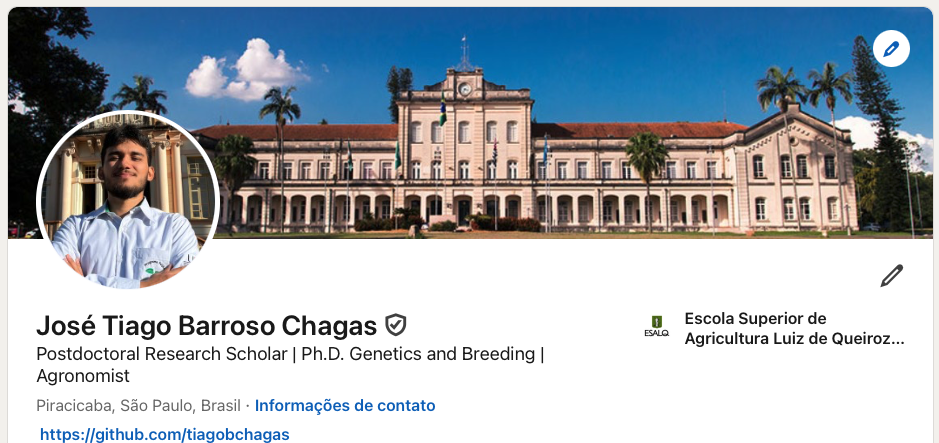
\includegraphics[width=0.58\linewidth,height=\textheight,keepaspectratio]{misc/linkedin.png}

\emph{Agronomist (\textbf{UFCA}- 2018)}

\emph{Msc. in Genetics and plant breeding (\textbf{UENF}-2020)}

\emph{Dsc. in Genetics and breeding (\textbf{UFV}- 2024)}

\emph{Postdoctoral research scholar (\textbf{UFV}-2024-2025);
(\textbf{ESALQ/USP}-2025)}
\end{frame}

\section{Experimental Design}\label{experimental-design}

\begin{frame}{Main principles of experimental design}
\phantomsection\label{main-principles-of-experimental-design}
\begin{figure}

\begin{minipage}{0.50\linewidth}

\begin{itemize}[<+->]
\tightlist
\item
  Replication
\item
  Randomization
\item
  Local control
\end{itemize}

\end{minipage}%
%
\begin{minipage}{0.50\linewidth}

\pandocbounded{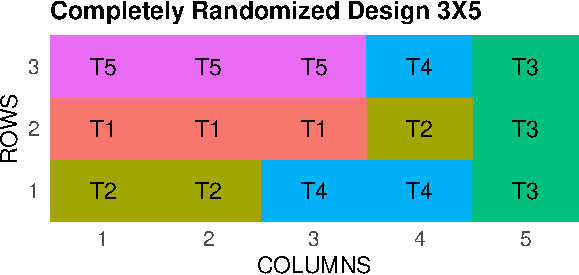
\includegraphics[keepaspectratio]{Sel_ind_files/figure-beamer/unnamed-chunk-1-1.pdf}}

\pandocbounded{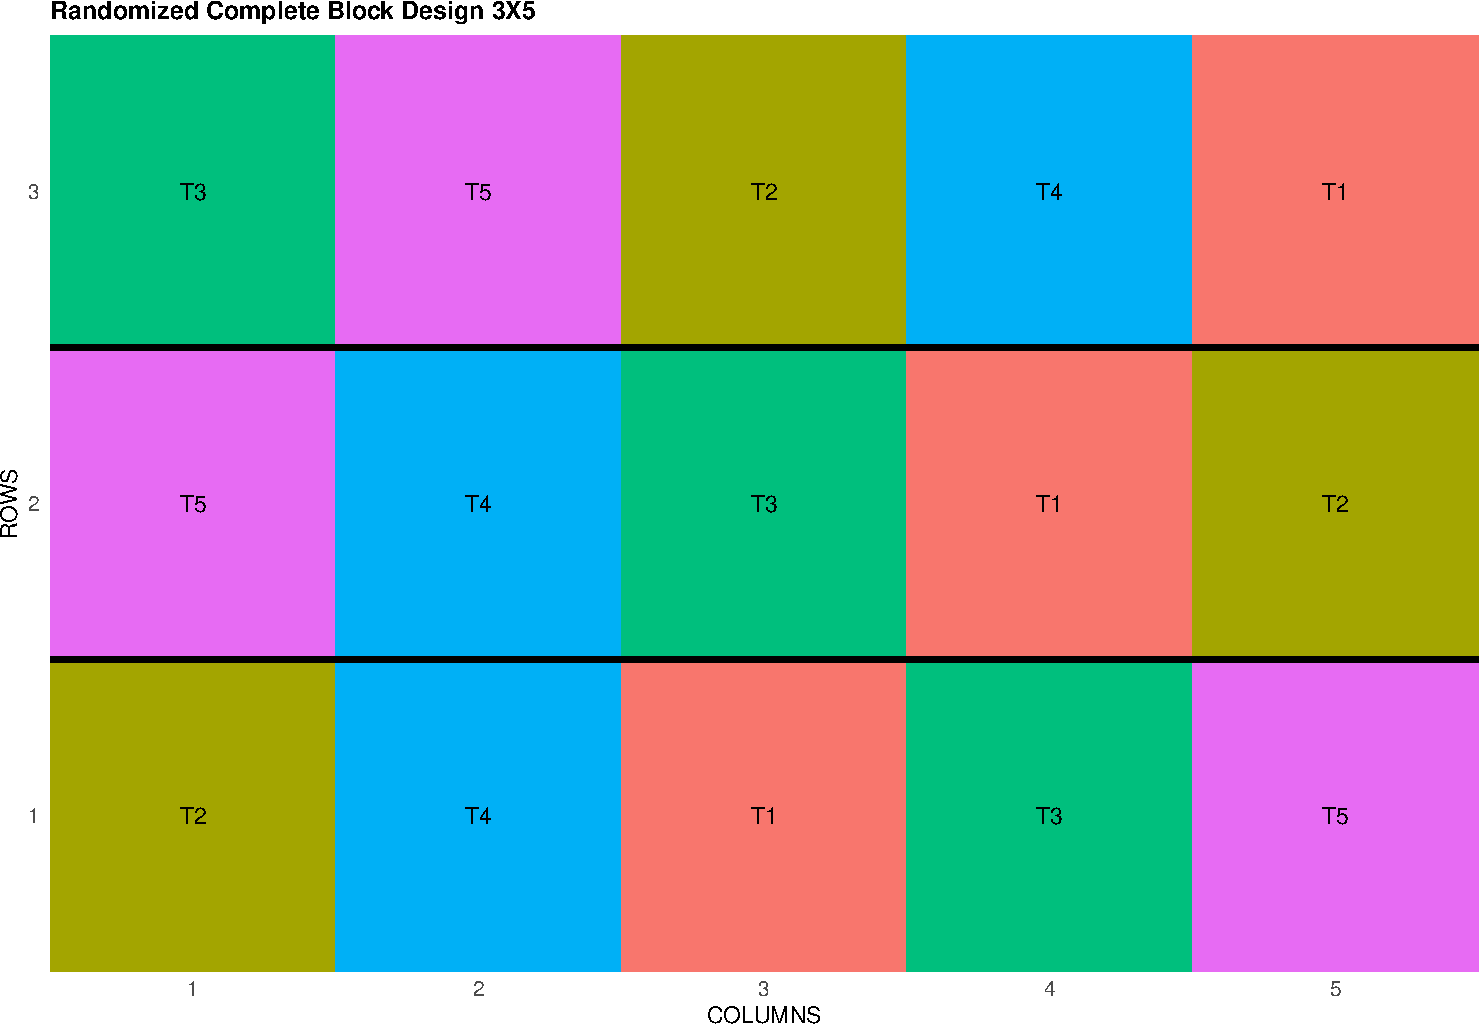
\includegraphics[keepaspectratio]{Sel_ind_files/figure-beamer/unnamed-chunk-1-2.pdf}}

\end{minipage}%

\end{figure}%
\end{frame}

\begin{frame}[fragile]{Square lattice}
\phantomsection\label{square-lattice}
\begin{columns}[T]
\begin{column}{0.25\linewidth}
\begin{itemize}[<+->]
\tightlist
\item
  Many test genotypes to evaluate in RCBD
\item
  \textbf{k} treatments by \textbf{k} blocks
\item
  (9treat/k3/rep3)
\end{itemize}
\end{column}

\begin{column}{0.75\linewidth}
\pandocbounded{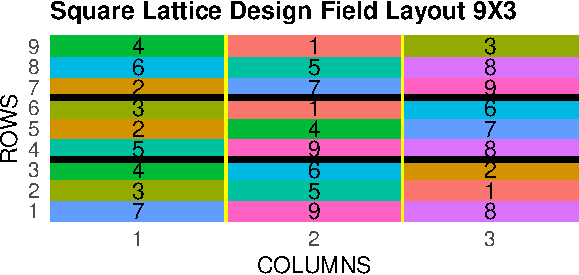
\includegraphics[keepaspectratio]{Sel_ind_files/figure-beamer/unnamed-chunk-2-1.pdf}}

\begin{verbatim}
  ID   LOCATION PLOT REP IBLOCK UNIT ENTRY TREATMENT
1  1 PIRACICABA 1001   1      1    1     7       G-7
2  2 PIRACICABA 1002   1      1    2     3       G-3
3  3 PIRACICABA 1003   1      1    3     4       G-4
\end{verbatim}
\end{column}
\end{columns}
\end{frame}

\begin{frame}[fragile]{Augmented randomized complete block design}
\phantomsection\label{augmented-randomized-complete-block-design}
\begin{columns}[T]
\begin{column}{0.3\linewidth}
\begin{itemize}[<+->]
\tightlist
\item
  Trials with few seeds available
\item
  Large number of treatments
\item
  (30gen/3check/k6)
\end{itemize}
\end{column}

\begin{column}{0.7\linewidth}
\begin{verbatim}
  ID   LOCATION PLOT ROW COLUMN CHECKS BLOCK ENTRY
1  1 PIRACICABA 1001   1      1      1     1     3
2  2 PIRACICABA 1002   1      2      1     1     2
3  3 PIRACICABA 1003   1      3      0     1    23
\end{verbatim}

\pandocbounded{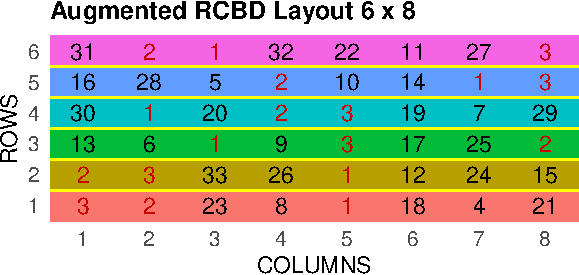
\includegraphics[keepaspectratio]{Sel_ind_files/figure-beamer/unnamed-chunk-3-1.pdf}}
\end{column}
\end{columns}
\end{frame}

\section{Mixed models equation}\label{mixed-models-equation}

\begin{frame}{Mixed models equation}
\phantomsection\label{mixed-models-equation-1}
\begin{columns}[T]
\begin{column}{0.65\linewidth}
Henderson (1953) (animal breeder) propose the mixed models equations.

Enables Best linear unbiased prediction (BLUP) and Best Linear Unbiased
Estimator (BLUE).
\end{column}

\begin{column}{0.35\linewidth}
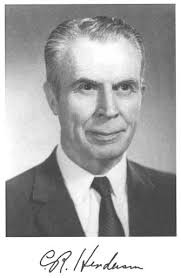
\includegraphics[width=0.58\linewidth,height=\textheight,keepaspectratio]{misc/henderso.jpeg}
\end{column}
\end{columns}
\end{frame}

\begin{frame}{Mixed models equation}
\phantomsection\label{mixed-models-equation-2}
\[
\textbf{y} = \mathbf{X}\beta + \mathbf{Z}u+ \mathbf{e}
\]

\[ 
\begin{bmatrix}
 \mathbf{X}'\mathbf{X} & \mathbf{X}'\mathbf{Z} \\
 \mathbf{Z}'\mathbf{X} & \mathbf{Z}'\mathbf{Z} + \lambda \mathbf{K}^{-1}
\end{bmatrix}
\begin{bmatrix}
 \mathbf{\hat{b}} \\
 \mathbf{\hat{u}}
\end{bmatrix}
=
\begin{bmatrix}
 \mathbf{X}'\mathbf{y} \\
 \mathbf{Z}'\mathbf{y}
\end{bmatrix}
\]

\begin{block}{Restricted maximum likelihood - (REML)}
\phantomsection\label{restricted-maximum-likelihood---reml}
Patterson and Thompson (1971) Restricted Maximum Likelihood (REML) of
random \(u\) and fixed effects \(\beta\).
\end{block}
\end{frame}

\begin{frame}{Maximum likelihood function}
\phantomsection\label{maximum-likelihood-function}
\[
f(x)= \frac{1}{\sigma \sqrt{2\pi}}e^{-\frac{1}{2}(\frac{x-\mu}{\sigma})^2}
\]

The maximum likelihood function seeks to optimize the values of the mean
\(\mu\) and variance \(\sigma\), given the observations and considering
normal distribution.
\end{frame}

\begin{frame}{Mixed models equation}
\phantomsection\label{mixed-models-equation-3}
Neste exemplo consideramos 100 valores aleatórios gerados de uma
distribuição normal com média 10 (\(\mu\)) e desvio padrão \(\sqrt{10}\)
(\(\sigma\))

\pandocbounded{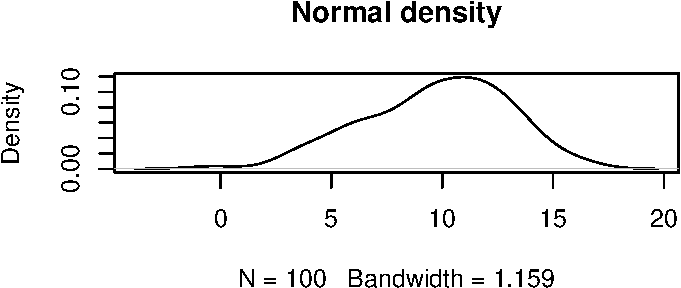
\includegraphics[keepaspectratio]{Sel_ind_files/figure-beamer/unnamed-chunk-4-1.pdf}}
\end{frame}

\begin{frame}{Maximum likelihood function}
\phantomsection\label{maximum-likelihood-function-1}
\begin{center}
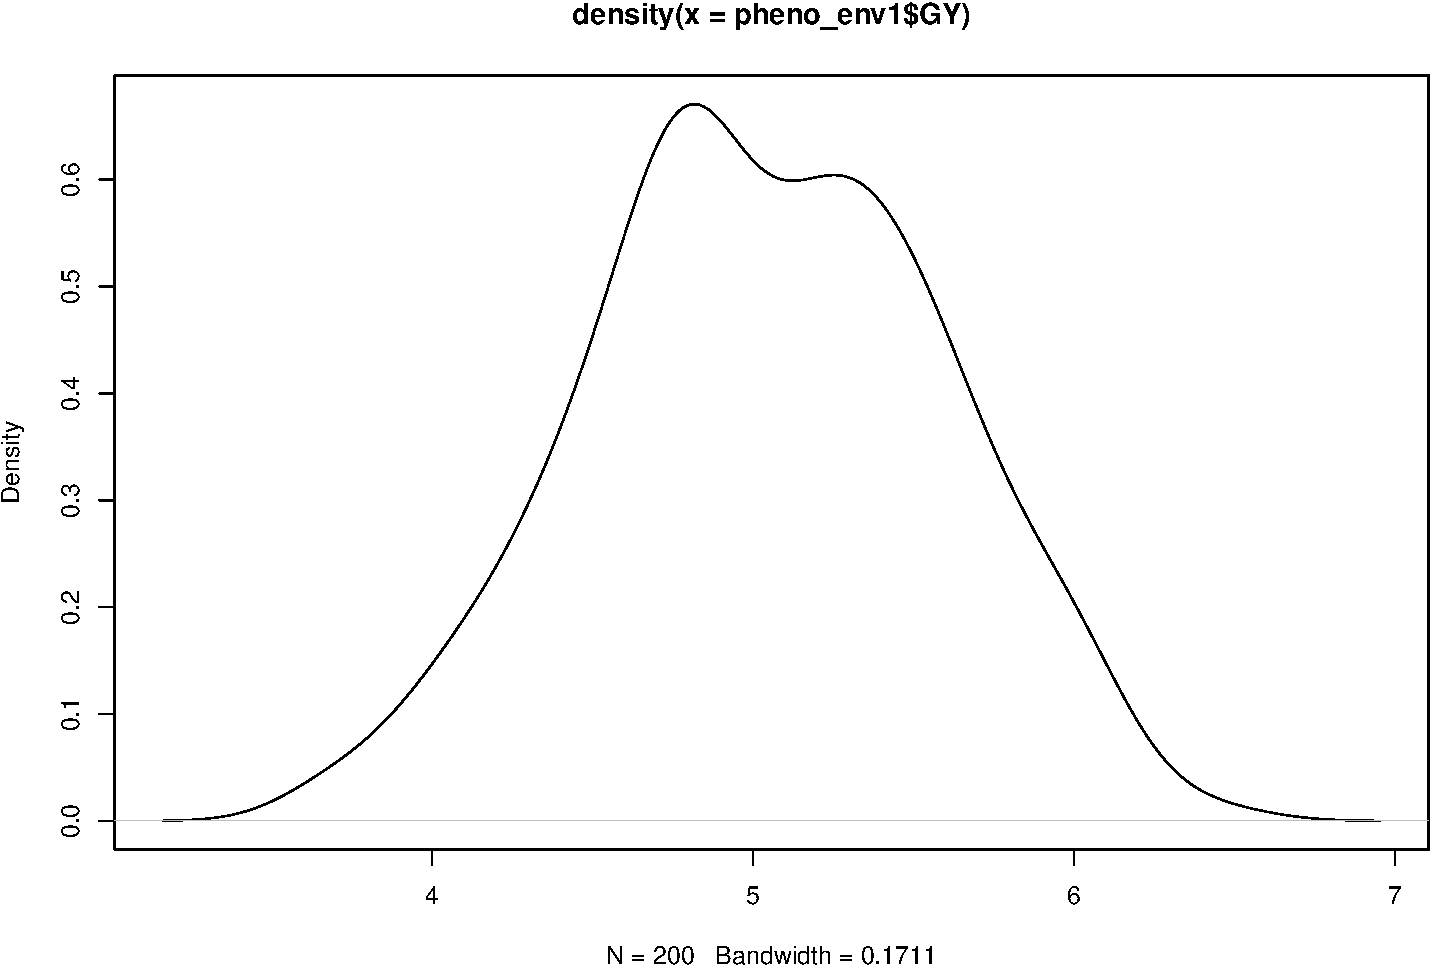
\includegraphics[width=0.6\linewidth,height=\textheight,keepaspectratio]{Sel_ind_files/figure-beamer/unnamed-chunk-5-1.pdf}
\end{center}
\end{frame}

\section{Single and Multienvironment
trials}\label{single-and-multienvironment-trials}

\begin{frame}{Simulating phenotypic traits}
\phantomsection\label{simulating-phenotypic-traits}
\begin{columns}[T]
\begin{column}{0.55\linewidth}
\begin{figure}[H]

{\centering \includegraphics[width=0.88\linewidth,height=\textheight,keepaspectratio]{misc/gy.jpeg}

}

\caption{Grain yield (kg ha⁻¹) of maize hybrids in simulated trials}

\end{figure}%
\end{column}

\begin{column}{0.45\linewidth}
\begin{figure}[H]

{\centering \includegraphics[width=0.48\linewidth,height=\textheight,keepaspectratio]{misc/ph.jpeg}

}

\caption{Plant Height (cm) of maize hybrids in simulated trials}

\end{figure}%
\end{column}
\end{columns}
\end{frame}

\begin{frame}{Simulating phenotypic traits}
\phantomsection\label{simulating-phenotypic-traits-1}
\begin{figure}

\begin{minipage}{0.50\linewidth}

\begin{figure}[H]

{\centering \pandocbounded{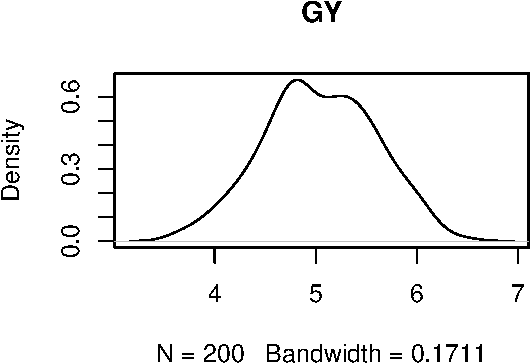
\includegraphics[keepaspectratio]{Sel_ind_files/figure-beamer/fig_simulated_traits-1.pdf}}

}

\subcaption{Grain Yield}

\end{figure}%

\end{minipage}%
%
\begin{minipage}{0.50\linewidth}

\begin{figure}[H]

{\centering \pandocbounded{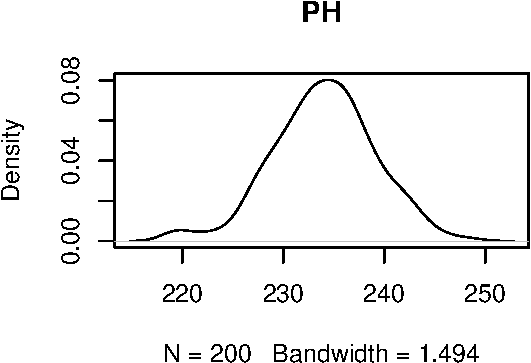
\includegraphics[keepaspectratio]{Sel_ind_files/figure-beamer/fig_simulated_traits-2.pdf}}

}

\subcaption{Plant height}

\end{figure}%

\end{minipage}%
\newline
\begin{minipage}{0.50\linewidth}
2 traits 100 genotypes 2 blocks\end{minipage}%

\end{figure}%
\end{frame}

\begin{frame}{Solving mixed models equation}
\phantomsection\label{solving-mixed-models-equation}
\[ 
\begin{bmatrix}
 \mathbf{X}'\mathbf{X} & \mathbf{X}'\mathbf{Z} \\
 \mathbf{Z}'\mathbf{X} & \mathbf{Z}'\mathbf{Z} + \lambda \mathbf{K}^{-1}
\end{bmatrix}
\begin{bmatrix}
 \mathbf{\hat{b}} \\
 \mathbf{\hat{u}}
\end{bmatrix}
=
\begin{bmatrix}
 \mathbf{X}'\mathbf{y} \\
 \mathbf{Z}'\mathbf{y}
\end{bmatrix}
\]

\begin{table}

\caption{\label{tbl-mixed-models}mixed models matrices}

\begin{minipage}{0.25\linewidth}

\subcaption{\label{tbl-mixed-models-1}X}

\centering{

\begin{tabular}{rr}
\toprule
block1 & block2\\
\midrule
1 & 0\\
1 & 0\\
1 & 0\\
\bottomrule
\end{tabular}

}

\end{minipage}%
%
\begin{minipage}{0.25\linewidth}

\subcaption{\label{tbl-mixed-models-2}Z}

\centering{

\begin{tabular}{rrr}
\toprule
id1 & id2 & id3\\
\midrule
0 & 0 & 0\\
0 & 0 & 0\\
0 & 0 & 0\\
\bottomrule
\end{tabular}

}

\end{minipage}%
%
\begin{minipage}{0.25\linewidth}

\subcaption{\label{tbl-mixed-models-3}y}

\centering{

\begin{tabular}{r}
\toprule
pheno\\
\midrule
5.513532\\
\bottomrule
\end{tabular}

}

\end{minipage}%
%
\begin{minipage}{0.25\linewidth}

\subcaption{\label{tbl-mixed-models-4}lambda}

\centering{

\begin{tabular}{rr}
\toprule
geno & erro\\
\midrule
0.0948 & 0.2075\\
\bottomrule
\end{tabular}

}

\end{minipage}%

\end{table}%
\end{frame}

\begin{frame}{Solving mixed models equation}
\phantomsection\label{solving-mixed-models-equation-1}
\begin{table}

\caption{\label{tbl-algebra}algebra with mixed models matrices}

\begin{minipage}{0.33\linewidth}

\subcaption{\label{tbl-algebra-1}XpX}

\centering{

\begin{tabular}{lrr}
\toprule
 & block1 & block2\\
\midrule
block1 & 100 & 0\\
block2 & 0 & 100\\
\bottomrule
\end{tabular}

}

\end{minipage}%
%
\begin{minipage}{0.33\linewidth}

\subcaption{\label{tbl-algebra-2}XpZ}

\centering{

\begin{tabular}{lrr}
\toprule
 & id1 & id2\\
\midrule
block1 & 1 & 1\\
block2 & 1 & 1\\
\bottomrule
\end{tabular}

}

\end{minipage}%
%
\begin{minipage}{0.33\linewidth}

\subcaption{\label{tbl-algebra-3}ZpX}

\centering{

\begin{tabular}{lrr}
\toprule
 & block1 & block2\\
\midrule
id1 & 1 & 1\\
id2 & 1 & 1\\
\bottomrule
\end{tabular}

}

\end{minipage}%
\newline
\begin{minipage}{0.33\linewidth}

\subcaption{\label{tbl-algebra-4}ZpZ}

\centering{

\begin{tabular}{lrr}
\toprule
 & id1 & id2\\
\midrule
id1 & 2 & 0\\
id2 & 0 & 2\\
\bottomrule
\end{tabular}

}

\end{minipage}%
%
\begin{minipage}{0.33\linewidth}

\subcaption{\label{tbl-algebra-5}Xpy}

\centering{

\begin{tabular}{lr}
\toprule
block1 & 498.0205\\
block2 & 509.2963\\
\bottomrule
\end{tabular}

}

\end{minipage}%
%
\begin{minipage}{0.33\linewidth}

\subcaption{\label{tbl-algebra-6}Zpy}

\centering{

\begin{tabular}{r}
\toprule
x\\
\midrule
8.834306\\
10.478144\\
\bottomrule
\end{tabular}

}

\end{minipage}%

\end{table}%
\end{frame}

\begin{frame}[fragile]{Solving mixed models equation}
\phantomsection\label{solving-mixed-models-equation-2}
\begin{figure}

\begin{minipage}{0.50\linewidth}

\begin{table}[H]

\caption{\label{tbl-lhs}LHS matrice}

\centering{

\begin{verbatim}
       block1 block2      id1
block1    100      0 1.000000
block2      0    100 1.000000
id1         1      1 4.188819
\end{verbatim}

}

\end{table}%

\end{minipage}%
%
\begin{minipage}{0.50\linewidth}

\begin{table}[H]

\caption{\label{tbl-rhs}RHS matrice}

\centering{

\begin{verbatim}
             [,1]
block1 498.020468
block2 509.296324
id1      8.834306
id2     10.478144
\end{verbatim}

}

\end{table}%

\end{minipage}%
\newline
\begin{minipage}{0.50\linewidth}

\begin{table}[H]

\caption{\label{tbl-sol}sol matrice}

\centering{

\begin{verbatim}
              [,1]
block1  4.98020468
block2  5.09296324
id1    -0.29575450
id2     0.09668033
\end{verbatim}

}

\end{table}%

\end{minipage}%

\end{figure}%
\end{frame}

\begin{frame}[fragile]{Solving mixed models equation (LME4)}
\phantomsection\label{solving-mixed-models-equation-lme4}
\begin{figure}

\begin{minipage}{0.50\linewidth}

\begin{verbatim}
Solving mixed models with package LME4
\end{verbatim}

\begingroup\fontsize{10}{12}\selectfont

\begin{longtable}[t]{r}

\caption{\label{tbl-rhs-lme4}RHS}

\tabularnewline

\\
\toprule
x\\
\midrule
-0.2957545\\
0.0966803\\
0.3478739\\
-0.0073687\\
-0.0808127\\
\addlinespace
-0.2544430\\
\bottomrule

\end{longtable}

\endgroup{}

\begin{verbatim}
[1] 4.980205 5.092963
\end{verbatim}

\end{minipage}%
%
\begin{minipage}{0.50\linewidth}

\begingroup\fontsize{10}{12}\selectfont

\begin{longtable}[t]{lr}

\caption{\label{tbl-lme4}LME4}

\tabularnewline

\\
\toprule
 & x\\
\midrule
id.(Intercept)1 & -0.3126610\\
id.(Intercept)2 & 0.1022069\\
id.(Intercept)3 & 0.3677597\\
id.(Intercept)4 & -0.0077899\\
id.(Intercept)5 & -0.0854323\\
\addlinespace
id.(Intercept)6 & -0.2689879\\
\bottomrule

\end{longtable}

\endgroup{}

\begin{verbatim}
(Intercept)        rep2 
  4.9802047   0.1127586 
\end{verbatim}

\end{minipage}%

\end{figure}%
\end{frame}

\begin{frame}{Multienvironmental trials}
\phantomsection\label{multienvironmental-trials}
\begin{figure}[H]

{\centering 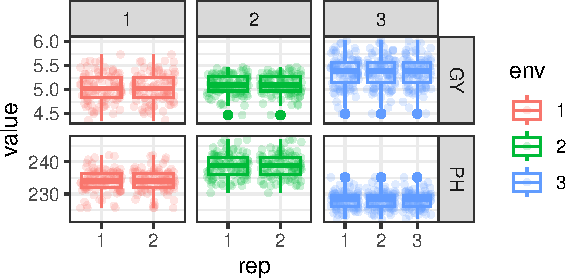
\includegraphics[width=0.3\linewidth,height=\textheight,keepaspectratio]{Sel_ind_files/figure-beamer/fig_multenv-1.pdf}

}

\caption{GY and PH evaluated in multenvironmental trials}

\end{figure}%

\[
\mathbf{y} = \mathbf{X}_1\mathbf{e} + \mathbf{X}_2\mathbf{be} + \mathbf{Z}_1\mathbf{g} + \mathbf{Z}_2\mathbf{ge} + \mathbf{\epsilon} 
\]

\([\mathbf{g}\sim N(0,\sigma_g^2\mathbf{I}_n)]\) and
\([\mathbf{ge}\sim N(0,\sigma_{ge}^2\mathbf{I}_{np})]\), where \(n\) is
the number of genotypes and \(p\) is the number of environments.
\end{frame}

\begin{frame}{Multienvironmental trials}
\phantomsection\label{multienvironmental-trials-1}
\textbf{2 traits; 100 genotypes; 2-3 blocks; 3 environments}

Testing genotype and genotype \(\times\) environment interaction effects
along traits.

\[
LRT = -2(LogL- LogL_{r})
\]

where \(LogL\) is the maximum point of the residual likelihood function
of the complete model and \(LogL_{r}\) is the same for the reduced model
\end{frame}

\begin{frame}[fragile]{Multienvironmental trials}
\phantomsection\label{multienvironmental-trials-2}
\begin{verbatim}
Data: pheno_df
Models:
mmcr: y.GY ~ env + rep:env + (1 | id)
mmc: y.GY ~ env + rep:env + (1 | id) + (1 | id:env)
     npar    AIC    BIC  logLik -2*log(L)  Chisq Df Pr(>Chisq)    
mmcr    9 1096.1 1137.0 -539.03    1078.1                         
mmc    10 1054.3 1099.8 -517.15    1034.3 43.758  1  3.717e-11 ***
---
Signif. codes:  0 '***' 0.001 '**' 0.01 '*' 0.05 '.' 0.1 ' ' 1
\end{verbatim}
\end{frame}

\begin{frame}{Multienvironmental trials}
\phantomsection\label{multienvironmental-trials-3}
\begin{figure}

\begin{minipage}{0.50\linewidth}

\begingroup\fontsize{10}{12}\selectfont

\begin{longtable}[t]{lr}
\caption{\label{tab:unnamed-chunk-7}LME4 - g x e}\\
\toprule
 & (Intercept)\\
\midrule
id:env.1:1 & -0.2994339\\
id:env.1:2 & -0.0883629\\
id:env.1:3 & 0.1092676\\
id:env.2:1 & 0.0992936\\
id:env.2:2 & -0.0491773\\
\addlinespace
id:env.2:3 & 0.0160696\\
\bottomrule
\end{longtable}
\endgroup{}

\end{minipage}%
%
\begin{minipage}{0.50\linewidth}

\begingroup\fontsize{10}{12}\selectfont

\begin{longtable}[t]{lr}
\caption{\label{tab:unnamed-chunk-8}LME4 - g}\\
\toprule
 & (Intercept)\\
\midrule
id.1 & -0.0803157\\
id.2 & 0.0218922\\
id.3 & 0.0822345\\
id.4 & 0.0073585\\
id.5 & 0.0976296\\
\addlinespace
id.6 & -0.0018268\\
\bottomrule
\end{longtable}
\endgroup{}

\end{minipage}%

\end{figure}%
\end{frame}

\begin{frame}{Multienvironmental trials}
\phantomsection\label{multienvironmental-trials-4}
\begin{figure}

\begin{minipage}{0.50\linewidth}

\begin{figure}[H]

{\centering \pandocbounded{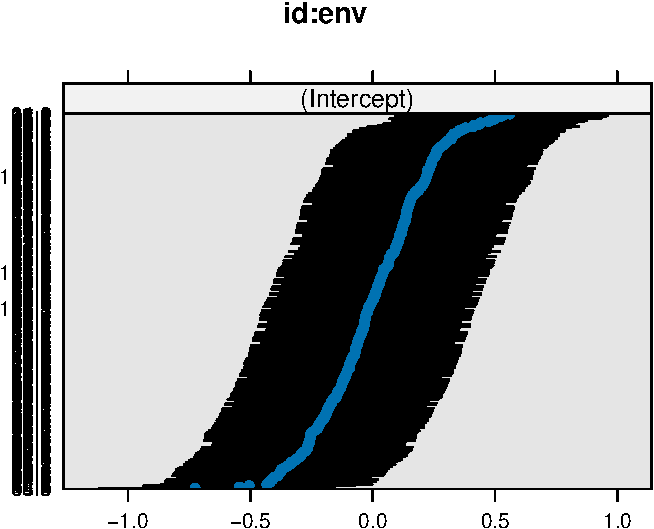
\includegraphics[keepaspectratio]{Sel_ind_files/figure-beamer/unnamed-chunk-9-1.pdf}}

}

\subcaption{modeling gxe}

\end{figure}%

\end{minipage}%
%
\begin{minipage}{0.50\linewidth}

\begin{figure}[H]

{\centering \pandocbounded{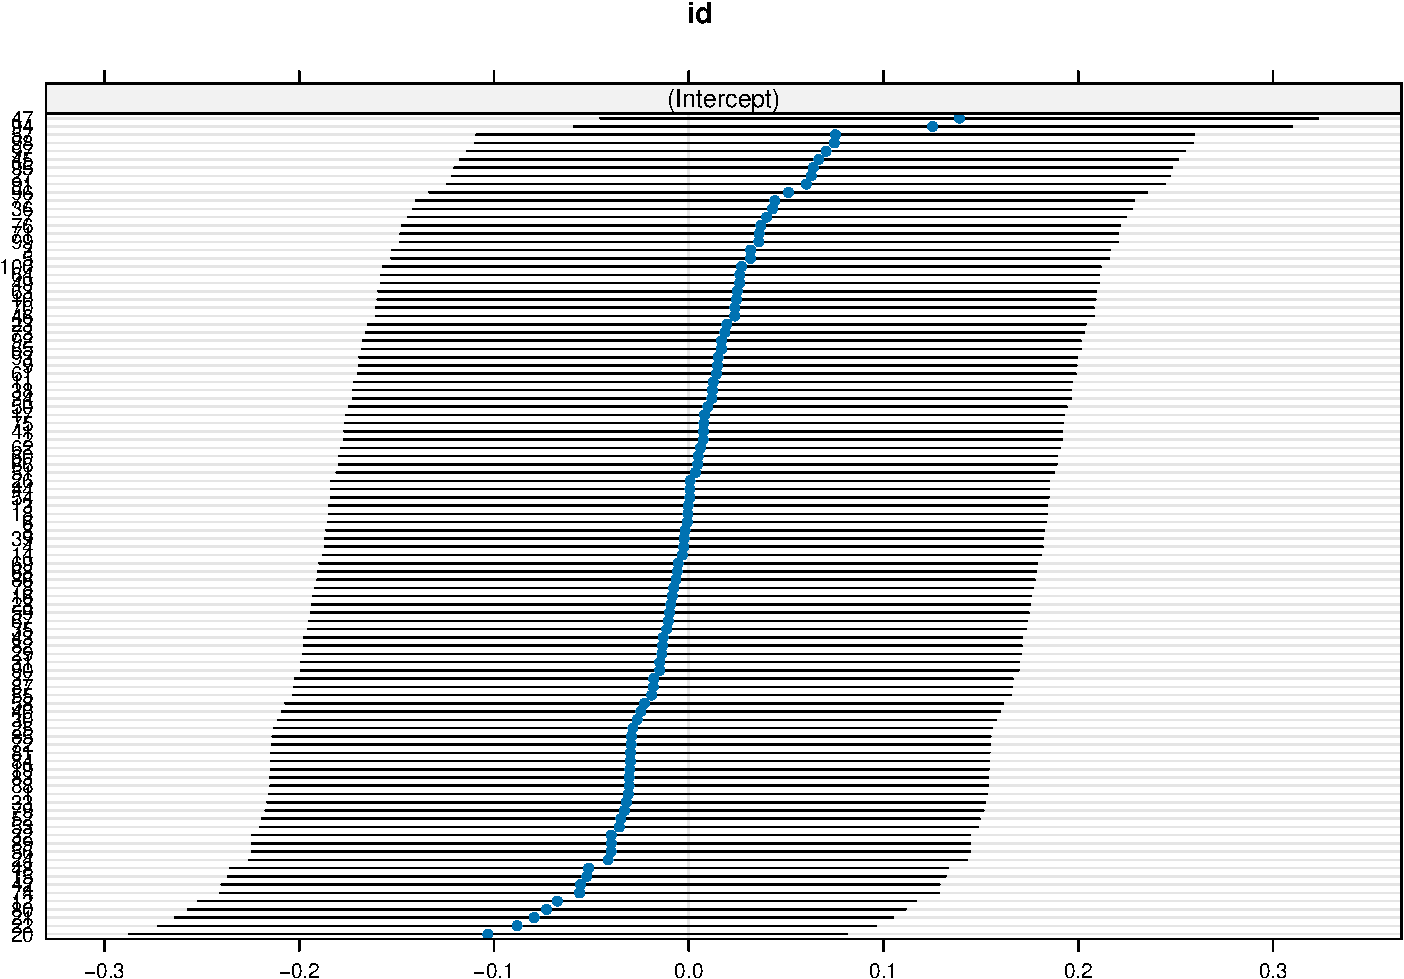
\includegraphics[keepaspectratio]{Sel_ind_files/figure-beamer/unnamed-chunk-9-2.pdf}}

}

\subcaption{ignoring gxe}

\end{figure}%

\end{minipage}%
\newline
\begin{minipage}{0.50\linewidth}
Predicition along multienvironmental trials\end{minipage}%

\end{figure}%
\end{frame}

\section{Selection indexes}\label{selection-indexes}

\begin{frame}{Selection indexes}
\phantomsection\label{selection-indexes-1}
\begin{block}{Indexes}
\phantomsection\label{indexes}
Several indexes were proposed with and without restrictions (Smith
(1936) \& Hazel (1943); Pešek and Baker (1969); Kempthorne and Nordskog
(1959)) and Bayesian probabilistic selection index (BPSI)(Chagas et al.
2025).
\end{block}
\end{frame}

\begin{frame}{Indexes}
\phantomsection\label{indexes-1}
\begin{block}{Smith e Hazel}
\phantomsection\label{smith-e-hazel}
\[
\hat{\underline{b}} = \hat{P}^{-1} \hat{G} \hat{a};\;
\] where \(\hat{P}\) and \(\hat{G}\) are phenotypic and genotypic
variance-covariance matrix, respectively, and \(\hat{a}\) are relative
economic values.
\end{block}

\begin{block}{Desire}
\phantomsection\label{desire}
\[
\underline{b} = G^{-1} \underline{q}
\] where \(G\) is the genotypic variance-covariance matrix and \(q\) is
the vector of desired gains (Pešek and Baker 1969)
\end{block}
\end{frame}

\begin{frame}{Desire and SH}
\phantomsection\label{desire-and-sh}
\begin{table}

\caption{\label{tbl-ds-sh}smith-hazel and desire indexes}

\begin{minipage}{0.33\linewidth}

\subcaption{\label{tbl-ds-sh-1}ebvMat}

\centering{

\begin{tabular}{lrr}
\toprule
 & PH\_1 & PH\_2\\
\midrule
39 & 238.25 & 239.84\\
4 & 226.52 & 232.95\\
\bottomrule
\end{tabular}

}

\end{minipage}%
%
\begin{minipage}{0.33\linewidth}

\subcaption{\label{tbl-ds-sh-2}Var\_Covar\_ebv}

\centering{

\begin{tabular}{rrrr}
\toprule
11.46 & 6.34 & 0.90 & -0.08\\
6.34 & 12.75 & -0.35 & 0.28\\
0.90 & -0.35 & 5.88 & 0.08\\
-0.08 & 0.28 & 0.08 & 0.09\\
\bottomrule
\end{tabular}

}

\end{minipage}%
%
\begin{minipage}{0.33\linewidth}

\subcaption{\label{tbl-ds-sh-3}economic weights}

\centering{

\begin{tabular}{r}
\toprule
x\\
\midrule
-1\\
-1\\
-1\\
2\\
2\\
2\\
\bottomrule
\end{tabular}

}

\end{minipage}%

\end{table}%
\end{frame}

\begin{frame}{Desire and SH}
\phantomsection\label{desire-and-sh-1}
\begin{table}

\caption{\label{tbl-ds-sh-results}results smith-hazel and desire}

\begin{minipage}{0.50\linewidth}

\subcaption{\label{tbl-ds-sh-results-1}economic weights}

\centering{

\begin{tabular}{r}
\toprule
0.3030121\\
-0.6317332\\
-0.7779787\\
6.9098122\\
15.9867062\\
3.9098938\\
\bottomrule
\end{tabular}

}

\end{minipage}%
%
\begin{minipage}{0.50\linewidth}

\subcaption{\label{tbl-ds-sh-results-2}optimum weights}

\centering{

\begin{tabular}{r}
\toprule
0.2303050\\
-0.6263726\\
-0.8032517\\
7.2542133\\
16.1879586\\
5.1908039\\
\bottomrule
\end{tabular}

}

\end{minipage}%

\end{table}%
\end{frame}

\begin{frame}{Desire and SH}
\phantomsection\label{desire-and-sh-2}
\begin{table}

\caption{\label{tbl-ds-sh-gain}weights smith-hazel and desire}

\begin{minipage}{0.25\linewidth}

\subcaption{\label{tbl-ds-sh-gain-1}gain SH}

\centering{

\begin{tabular}{lr}
\toprule
 & x\\
\midrule
PH\_1 & 0.3386552\\
PH\_2 & 0.5247615\\
PH\_3 & -0.6109782\\
GY\_1 & 0.3010492\\
GY\_2 & 0.2870106\\
GY\_3 & 0.2522658\\
\bottomrule
\end{tabular}

}

\end{minipage}%
%
\begin{minipage}{0.25\linewidth}

\subcaption{\label{tbl-ds-sh-gain-2}SH}

\centering{

\begin{tabular}{r}
\toprule
x\\
\midrule
1.262474\\
\bottomrule
\end{tabular}

}

\end{minipage}%
%
\begin{minipage}{0.25\linewidth}

\subcaption{\label{tbl-ds-sh-gain-3}gain DS}

\centering{

\begin{tabular}{lr}
\toprule
 & x\\
\midrule
PH\_1 & 0.2606474\\
PH\_2 & 0.5924429\\
PH\_3 & -0.6445062\\
GY\_1 & 0.2488413\\
GY\_2 & 0.2344179\\
GY\_3 & 0.2209354\\
\bottomrule
\end{tabular}

}

\end{minipage}%
%
\begin{minipage}{0.25\linewidth}

\subcaption{\label{tbl-ds-sh-gain-4}DS}

\centering{

\begin{tabular}{r}
\toprule
x\\
\midrule
1.380423\\
\bottomrule
\end{tabular}

}

\end{minipage}%

\end{table}%
\end{frame}

\begin{frame}{Índice de Seleção}
\phantomsection\label{uxedndice-de-seleuxe7uxe3o}
\[
P_{ij} = \frac{\frac{1}{d_{ij}}}{\sum^{i=n;j=m}_{i=1;j=1} \frac{1}{d_{ij}}}
\]

\(P_{ij}\) probabilidade do i-ésimo genótipo ser similar ao j-ésimo
ideótipo, \(d_{ij}\) distância genótipo-ideótipo euclidiana padronizada.
\end{frame}

\section{Bayesian probabilistic selection index
(BPSI)}\label{bayesian-probabilistic-selection-index-bpsi}

\begin{frame}{Hypothesis}
\phantomsection\label{hypothesis}
\begin{block}{\textbf{Hypothesis}}
\begin{itemize}
\item Probability of superior performance (Dias \textit{et al.}, 2022)  \\~\\
\item Selection Index (Classify progenies)
\end{itemize}
\end{block}
\end{frame}

\begin{frame}{Goals}
\phantomsection\label{goals}
\begin{itemize}
\item i) extend the probabilistic method to a selection index (BPSI) 
\item ii) select families from carioca common bean recurrent selection to extract pure lines using BPSI index.
\end{itemize}
\end{frame}

\begin{frame}{Bayesian Probabilistic selection index}
\phantomsection\label{bayesian-probabilistic-selection-index}
BPSI index uses the probability of superior performance to estimate the
chance of a genotype being selected in multienvironmental trials Dias et
al. (2022).

\[
Pr\left({\hat{g}}_i \in \Omega \middle| y\right) = \frac{1}{s}\sum_{s=1}^{s} I \left({\hat{g}}_i^{(s)} \in \Omega \middle| y\right) \tag{1}
\]

where \(\hat{g}_i\) is the genotypic value, \(\Omega\) is a subset of
genotypes with superior performance and \(s\) represents each sample of
posterior distribution.
\end{frame}

\begin{frame}{Bayesian Probabilistic selection index}
\phantomsection\label{bayesian-probabilistic-selection-index-1}
\[
BPSI_i = \sum_{m = 1}^t \frac{RankProbSup}{\omega}
\]

where \(t\) is the total number of traits evaluated
\((m = 1, 2, \ldots, t)\) and \(\omega\) is a weight. Traits of greater
interest will have larger ω. We used weight 2 for GY and weight 1 for
CGA and PA. The 10\% best-ranked families were selected according to the
BPSI.

\begin{table}

\caption{\label{tbl-table1}Hypothetical scheme of three genotypes
evaluated for three traits}

\centering{

\centering\begingroup\fontsize{10}{12}\selectfont

\begin{tabular}{l|l|l|l|l}
\hline
Genotype & T1(Rank) & T2(Rank) & T3(Rank) & BPSI\\
\hline
1 & 10 & 5 & 2 & ∑ i. = 17\\
\hline
2 & 5 & 3 & 10 & ∑ i. = 18\\
\hline
3 & 7 & 3 & 10 & ∑ i. = 19\\
\hline
\end{tabular}
\endgroup{}

}

\end{table}%
\end{frame}

\begin{frame}{Bayesian Probabilistic selection index}
\phantomsection\label{bayesian-probabilistic-selection-index-2}
Probability of superior performance within environments

\[
Pr\left(\widehat{g_{ij}} \in \Omega_j \middle| y\right) = \frac{1}{S}\sum_{s=1}^{S} I\left(\widehat{g_{ij}^{(s)}} \in \Omega_j \middle| y\right)
\]

Pairwise probability of superior performance

\[
Pr\left(\widehat{g_i} > \widehat{g_{i^\prime}} \middle| y\right) = \frac{1}{S}\sum_{s=1}^{S} I\left(\widehat{g_i^{(s)}} > \widehat{g_{i^\prime}^{(s)}} \middle| y\right)
\]
\end{frame}

\begin{frame}{Plant material and experimental design}
\phantomsection\label{plant-material-and-experimental-design}
\begin{figure}[H]

{\centering 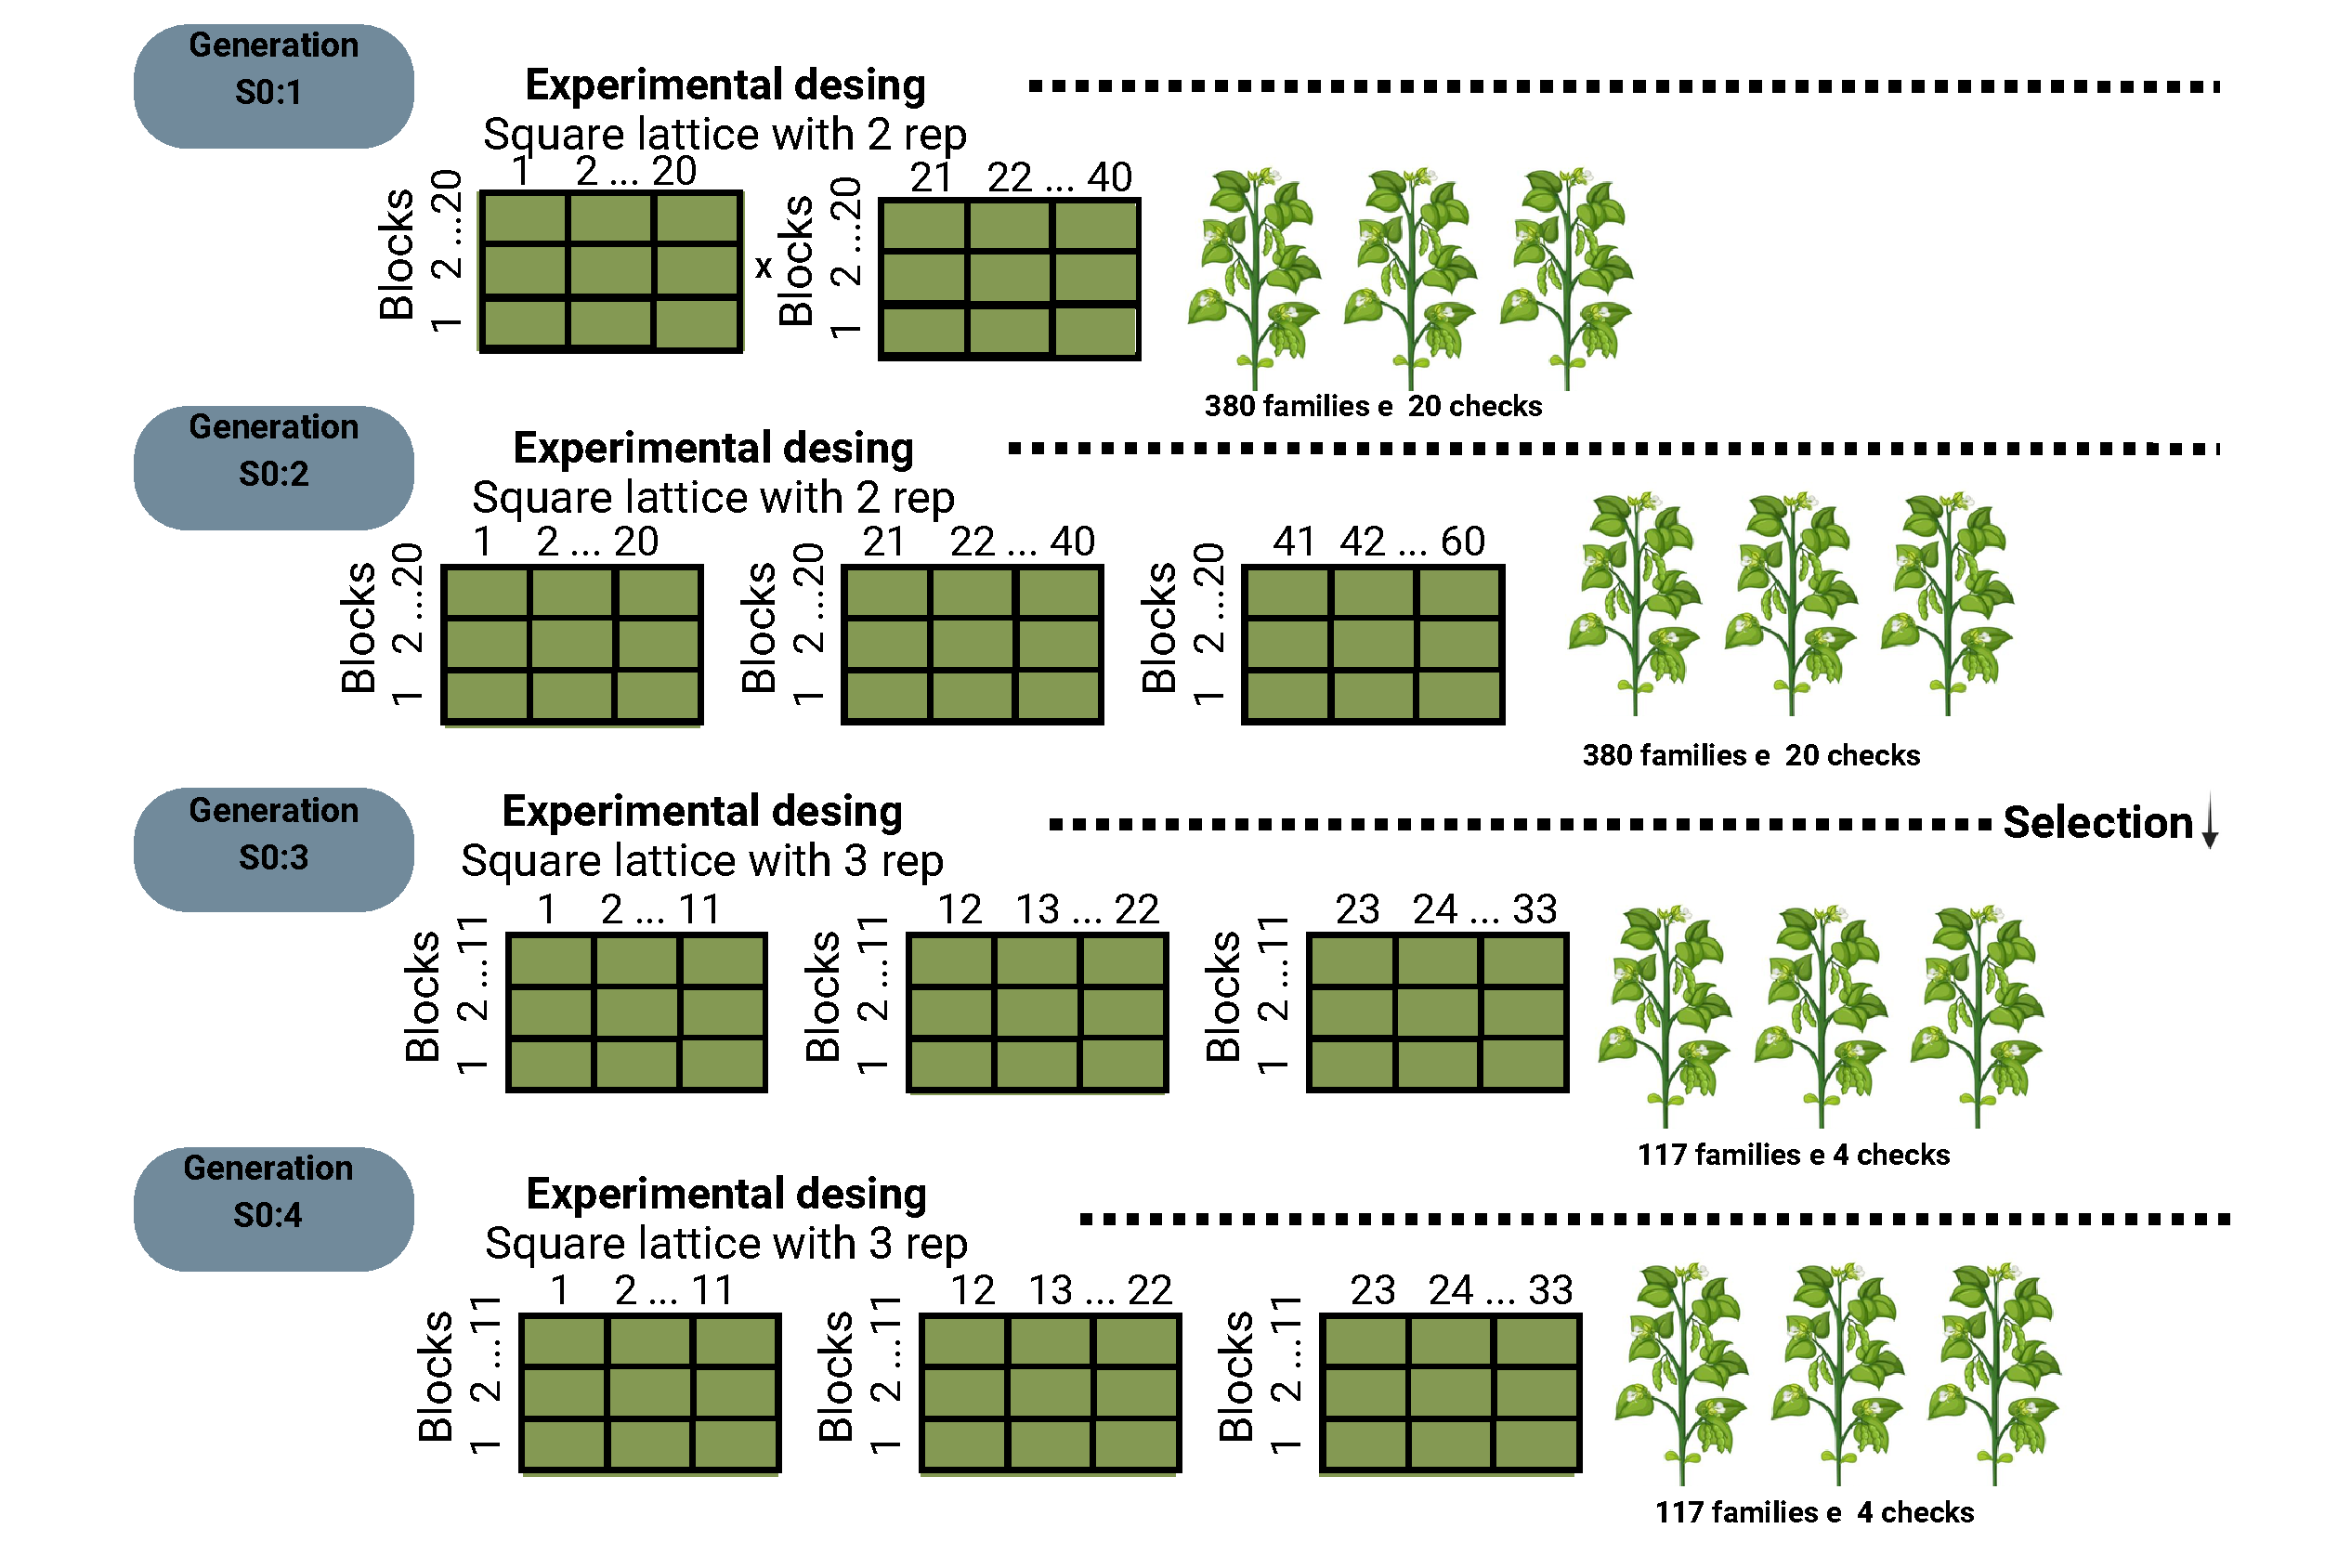
\includegraphics[width=0.65\linewidth,height=\textheight,keepaspectratio]{misc/images/experimental design.pdf}

}

\caption{Experimental design}

\end{figure}%
\end{frame}

\begin{frame}{Traits evaluated}
\phantomsection\label{traits-evaluated}
\begin{columns}[T]
\begin{column}{0.32\linewidth}
\begin{figure}

\centering{

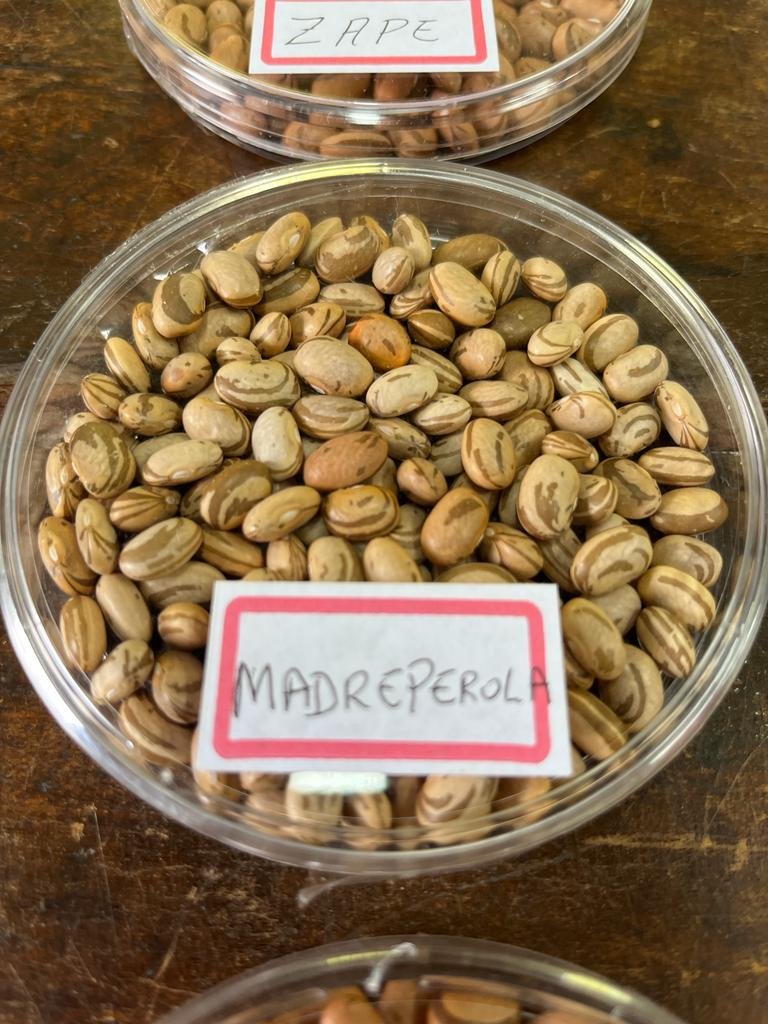
\includegraphics[width=0.55\linewidth,height=\textheight,keepaspectratio]{misc/images/acg.jpg}

}

\caption{\label{fig-acg}Commercial Grain Appearance}

\end{figure}%
\end{column}

\begin{column}{0.32\linewidth}
\begin{figure}

\centering{

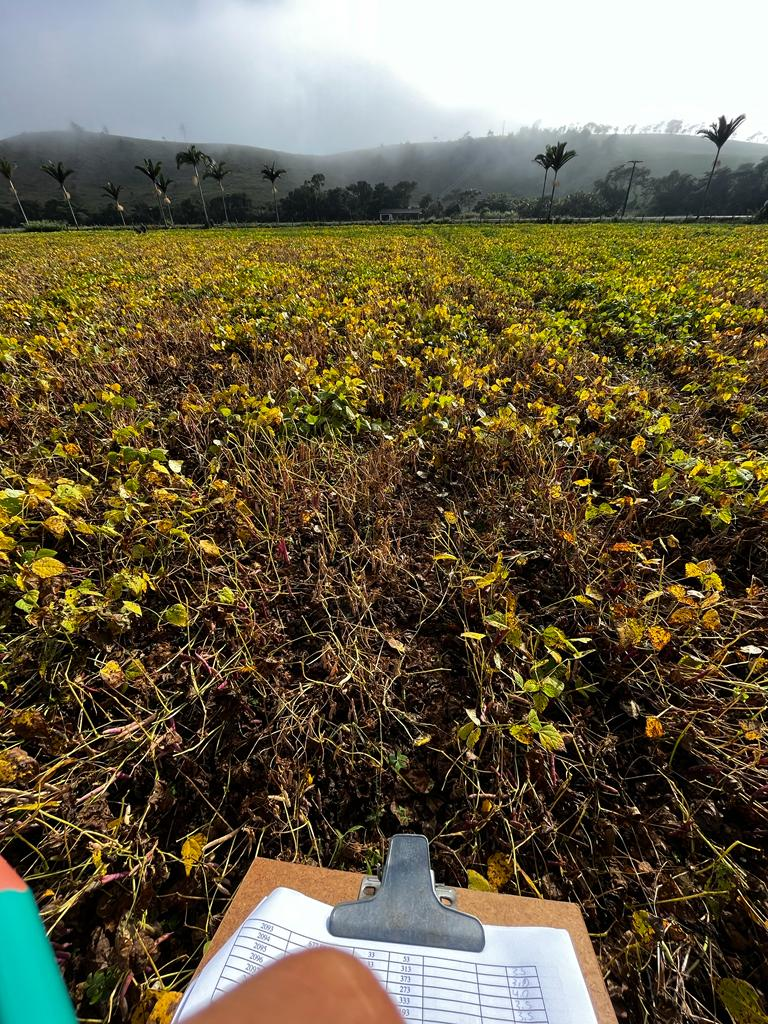
\includegraphics[width=0.55\linewidth,height=\textheight,keepaspectratio]{misc/images/arq.jpg}

}

\caption{\label{fig-arq}Plant Architecture}

\end{figure}%
\end{column}

\begin{column}{0.32\linewidth}
\begin{figure}

\centering{

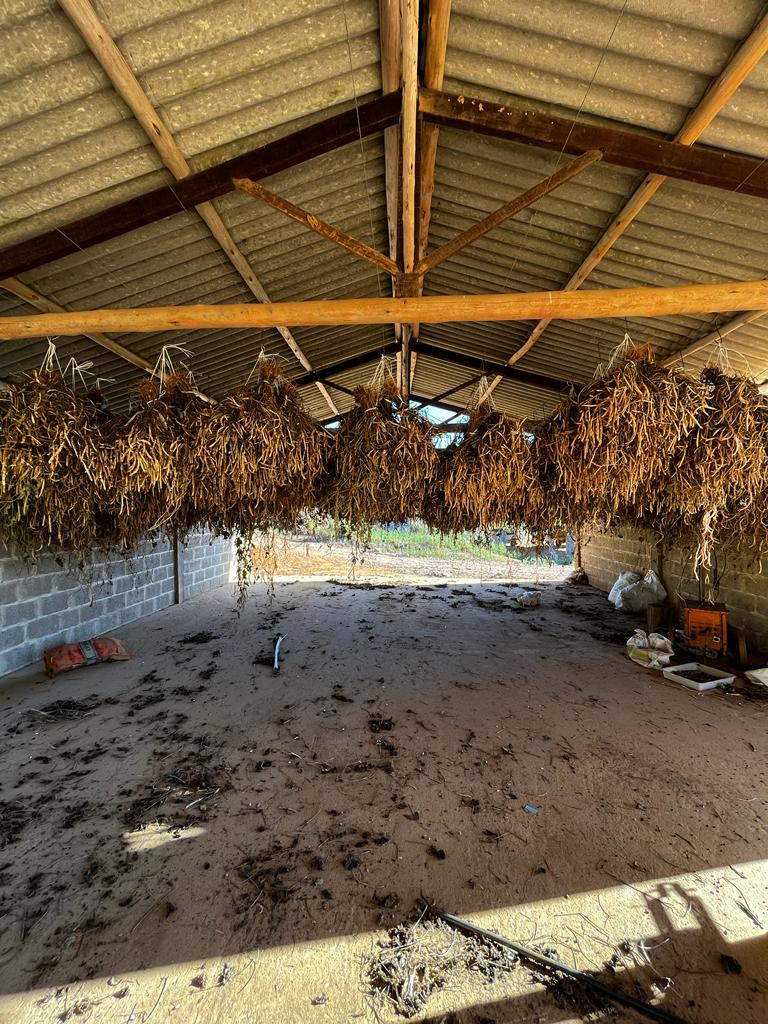
\includegraphics[width=0.55\linewidth,height=\textheight,keepaspectratio]{misc/images/prod.jpg}

}

\caption{\label{fig-prod}Grain Yield}

\end{figure}%
\end{column}
\end{columns}
\end{frame}

\begin{frame}{First step: Adjusted means}
\phantomsection\label{first-step-adjusted-means}
Individual analysis was realized in each trial to get genotypes adjusted
means:

\[
 \mathbf{Y} = \mathbf{X}_{1}\mathbf{r} + \mathbf{X}_{2}\mathbf{g} + \mathbf{Z}\mathbf{b} + \boldsymbol{\epsilon}
\]

where \(\mathbf{Y}_{(n\times1)}\) is vector of observations,
\(\mathbf{X_1}_{(n \times r)}\) is a incidence matrix \(\textbf{r}\) of
replication effect assumed as fixed, \(\mathbf{X_2}_{(n\times rk)}\) is
a incidence matrix \(\textbf{g}\) of genotype effect assumed as fixed,
\(\mathbf{Z}_{(n\times k)}\) is a incidence matrix \(\textbf{k}\) of
block effect assumed as random and
\(\mathbf{\varepsilon}_{(n\times 1)}\) is a vector of random errors.

The variance probability density related to model terms are:
\(\textbf{b} \sim N (0,\sigma_{b}^{2}\mathbf{I}_k)\)
\end{frame}

\begin{frame}{Second step: Bayesian model}
\phantomsection\label{second-step-bayesian-model}
The probabilistic model proposed by Dias et al. (2022) was fitted to
each trait and setting priors to variance components of genotype,
environment, and \((G\times E)\) interaction.

\[
E[{Y}_{ij}] = {\mu} + {g}_i + {a}_j + {(ga)}_{ij} + {\epsilon}_{ij}
\]

where \(E[{Y}_{ij}]\) is expectation of observation \(ij\), \({g}_{i}\)
is the effect \(i\) of genotypes assumed as random (\(i^{th}\) = 121
genotypes), \({a}_{j}\) is the effect \(j\) of environment assumed as
random (\(j^{th}\) = 4 environments), \({ga}_{ij}\) is the effect of
\((G\times E)\) interaction assumed as random and \({\varepsilon}\) is
the effect of random errors.
\end{frame}

\begin{frame}{Priori}
\phantomsection\label{priori}
Prior distribution was normal density and the variance probability
density related to model terms are:

\[{g}_i \sim N (0,{S}^{[g]})\]

\[{a}_j \sim N (0,{S}^{[a]})\]

\[{(ga)}_{ij} \sim N (0,{S}^{[ga]})\]

\[{\sigma} \sim HalfCauchy (0,{S}^{[\sigma]})\]
\end{frame}

\begin{frame}{Priori}
\phantomsection\label{priori-1}
Parameters of prior distribution was assumed as hyperparameters:

\[ {S}^{[{g}]} \sim \textit{HalfCauchy} (0,\phi) \]

\[ {S}^{[{a}]} \sim \textit{HalfCauchy} (0,\phi) \]

\[ {S}^{[{ga}]} \sim \textit{HalfCauchy} (0,\phi) \]
\end{frame}

\begin{frame}{Bayesian variance components}
\phantomsection\label{bayesian-variance-components}
\begingroup\fontsize{8}{10}\selectfont

\begin{longtable}[t]{llrrr}

\caption{\label{tbl-variance-components}Common bean UFV carioca
population variance components for different traits at trials from 2020
to 2023}

\tabularnewline

\\
\toprule
trait & effect & var & HPD\_0.025 & HPD\_0.975\\
\midrule
GA & genotype & 0.031 & 0.018 & 0.047\\
GA & environment & 8.136 & 0.009 & 20.868\\
GA & gen.env & 0.040 & 0.000 & 0.081\\
GA & error & 0.036 & 0.002 & 0.082\\
GY & genotype & 18314.900 & 332.149 & 42239.694\\
\addlinespace
GY & environment & 3808551.300 & 143501.463 & 21978738.500\\
GY & gen.env & 32543.119 & 1.586 & 156390.836\\
GY & error & 193951.014 & 69921.263 & 256589.277\\
PA & genotype & 0.035 & 0.019 & 0.053\\
PA & environment & 180.519 & 0.150 & 1020.549\\
\addlinespace
PA & gen.env & 0.018 & 0.000 & 0.045\\
PA & error & 0.032 & 0.007 & 0.059\\
\bottomrule

\end{longtable}

\endgroup{}
\end{frame}

\begin{frame}{Bayesian model fitting}
\phantomsection\label{bayesian-model-fitting}
\begin{figure}[H]

{\centering 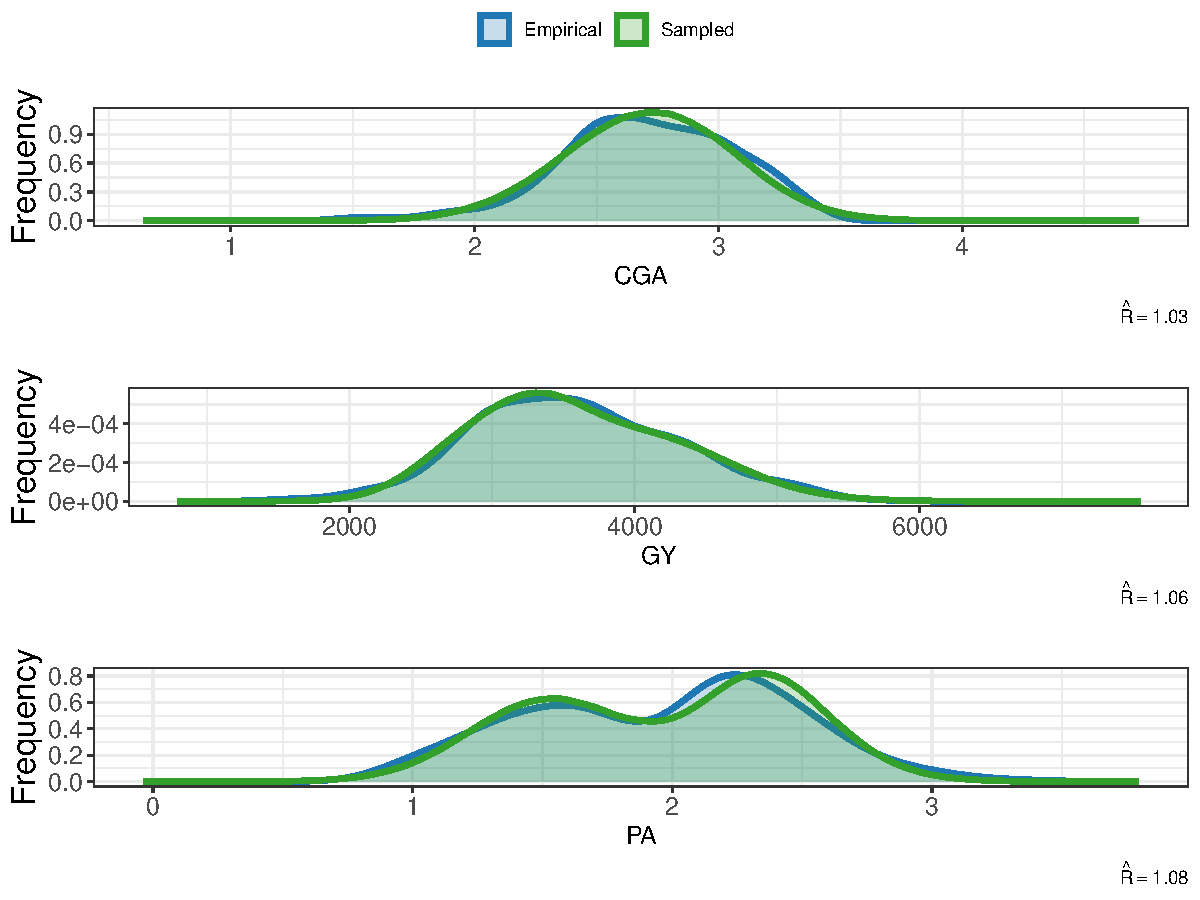
\includegraphics[width=0.6\linewidth,height=\textheight,keepaspectratio]{misc/images/PlotsDen.pdf}

}

\caption{Bayesian model fitting results}

\end{figure}%
\end{frame}

\begin{frame}{Probability of superior performance across environments}
\phantomsection\label{probability-of-superior-performance-across-environments}
\begin{figure}[H]

{\centering 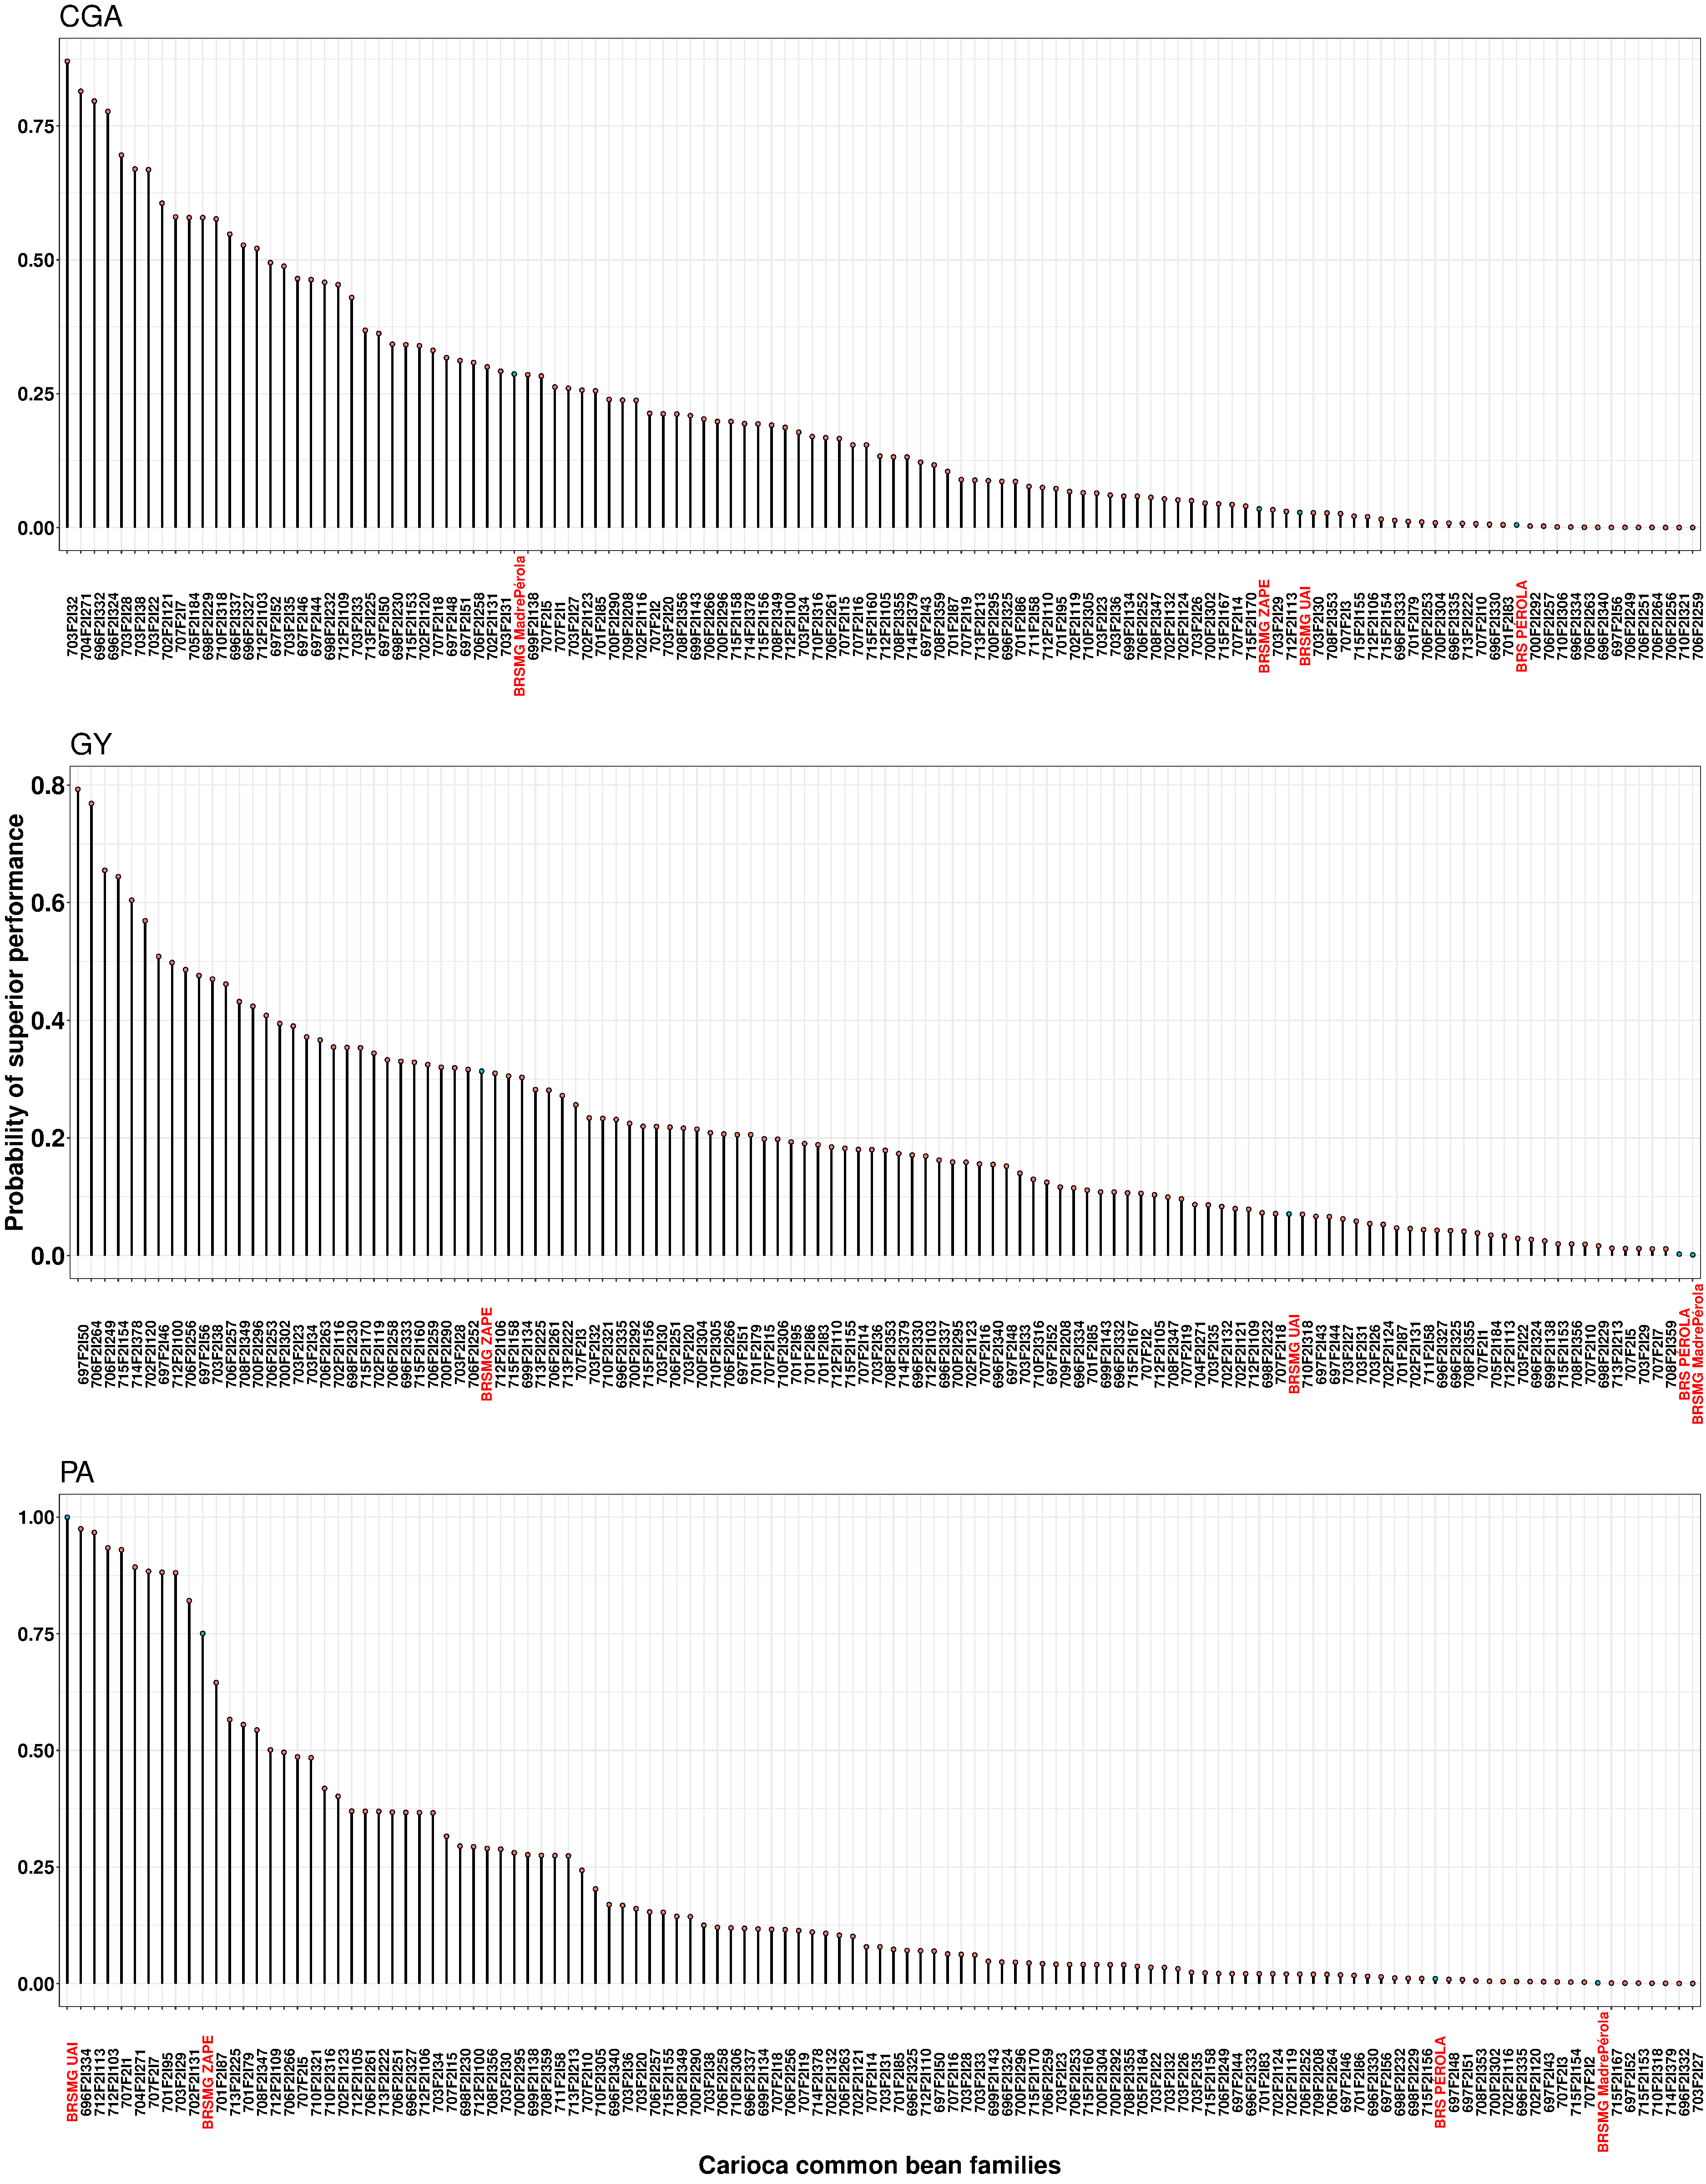
\includegraphics[width=0.35\linewidth,height=\textheight,keepaspectratio]{misc/images/PlotsMargs.pdf}

}

\caption{Probability of superior performance across environments}

\end{figure}%
\end{frame}

\begin{frame}{Probability of superior performance within environments}
\phantomsection\label{probability-of-superior-performance-within-environments}
\begin{figure}[H]

{\centering 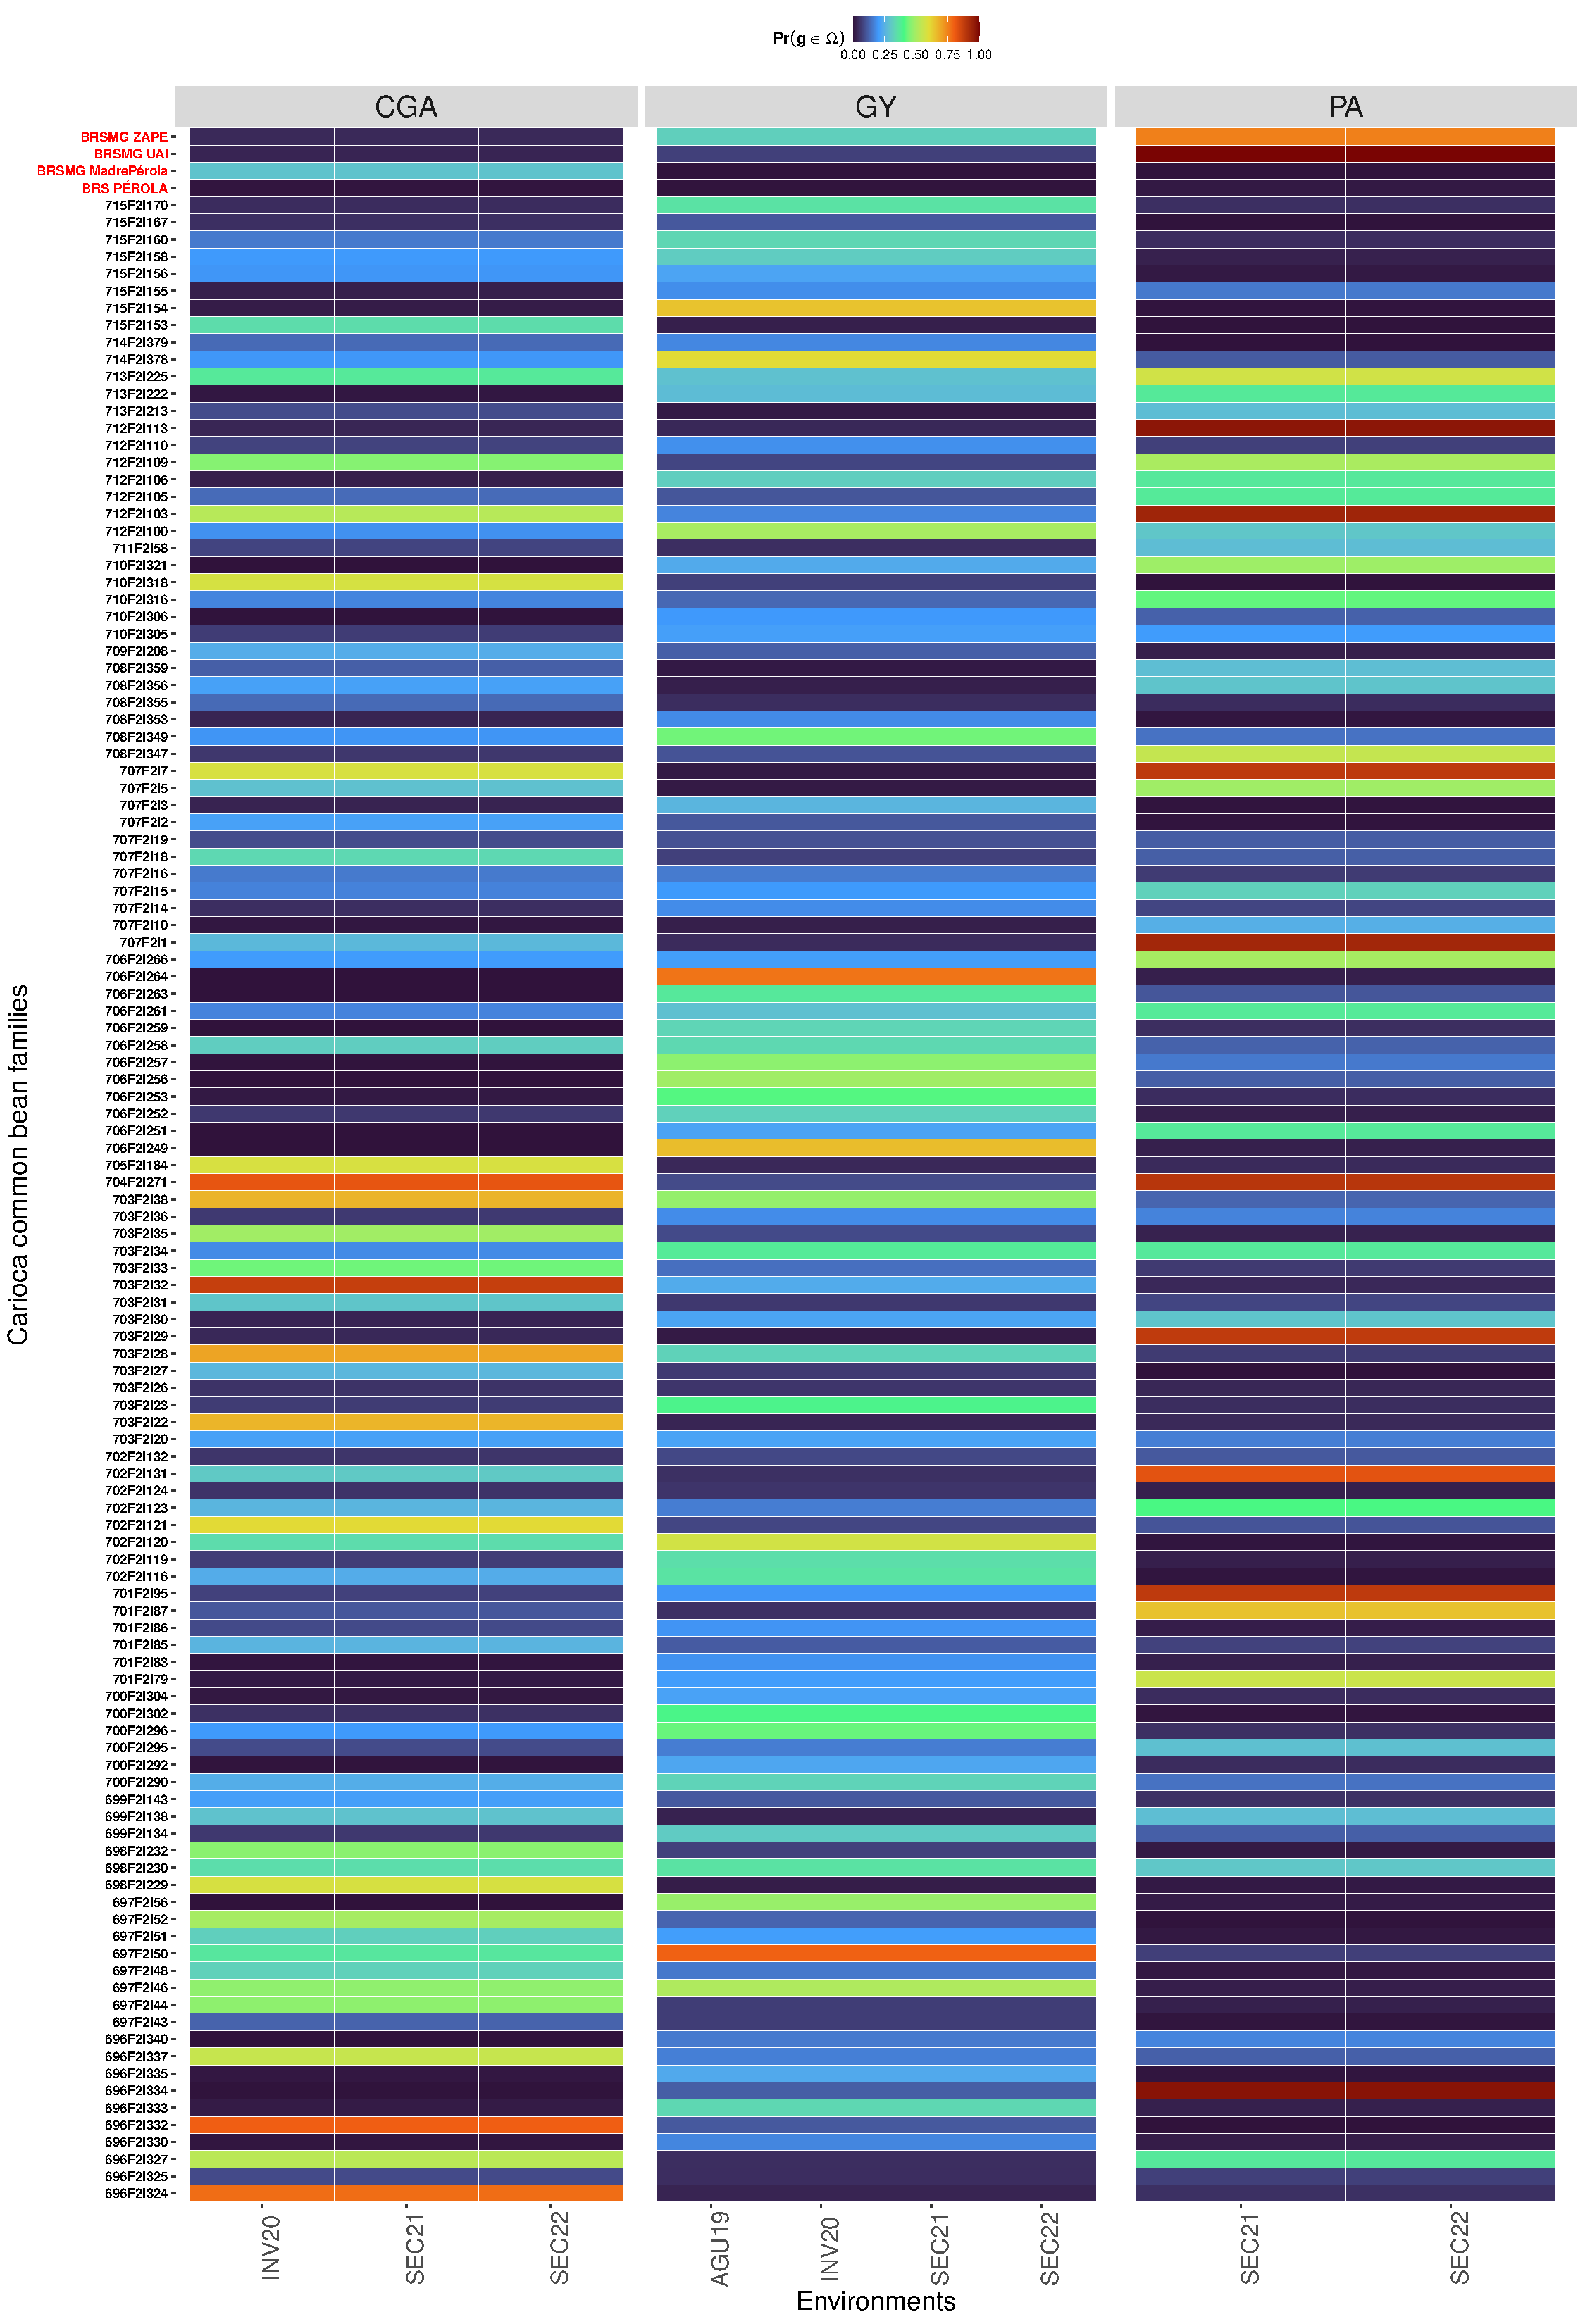
\includegraphics[width=0.3\linewidth,height=\textheight,keepaspectratio]{misc/images/PlotsConds.pdf}

}

\caption{Probability of superior performance within environments}

\end{figure}%
\end{frame}

\begin{frame}{Pairwise probability of superior performance}
\phantomsection\label{pairwise-probability-of-superior-performance}
\begin{figure}[H]

{\centering 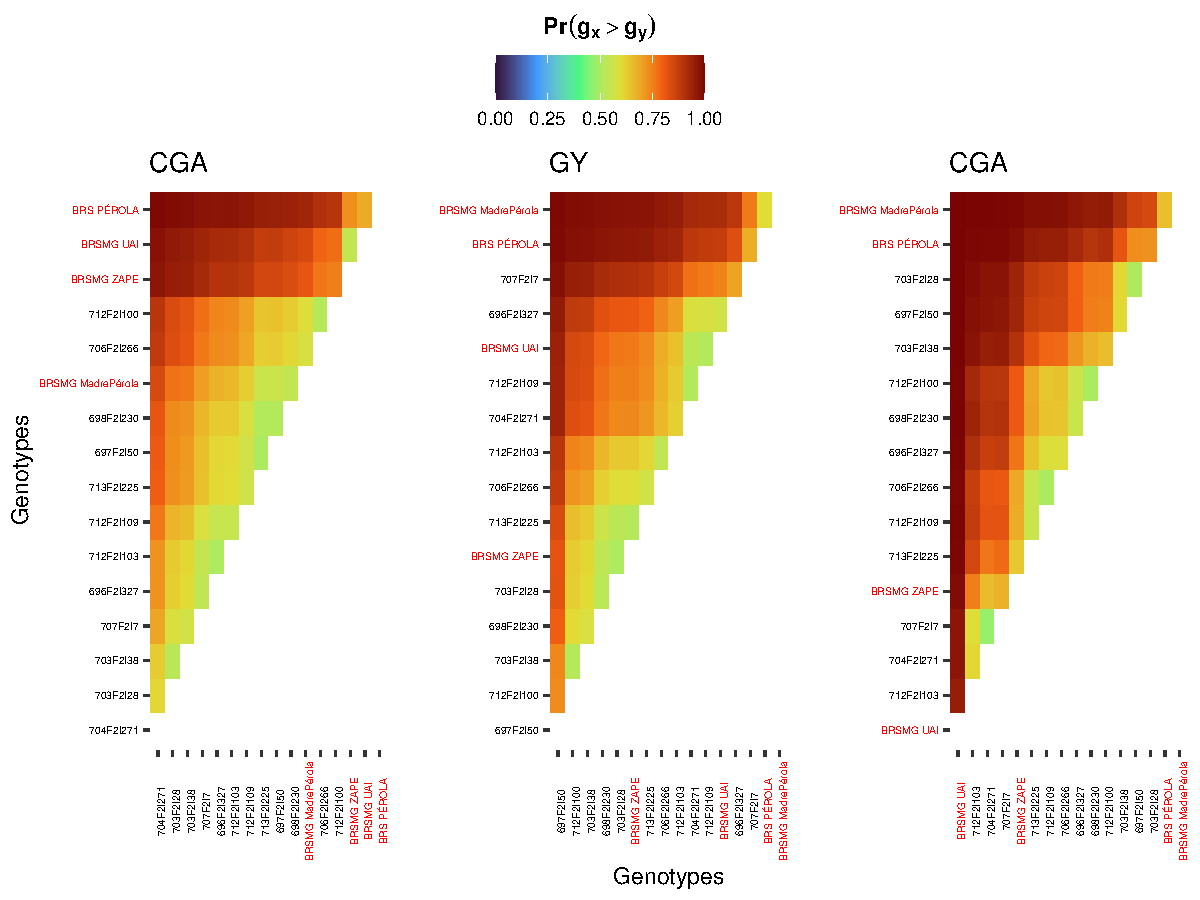
\includegraphics[width=0.6\linewidth,height=\textheight,keepaspectratio]{misc/images/PlotsPairs.pdf}

}

\caption{Pairwise probability of superior performance}

\end{figure}%
\end{frame}

\begin{frame}{Bayesian Probabilistic Selection Index}
\phantomsection\label{bayesian-probabilistic-selection-index-3}
\begin{figure}[H]

{\centering 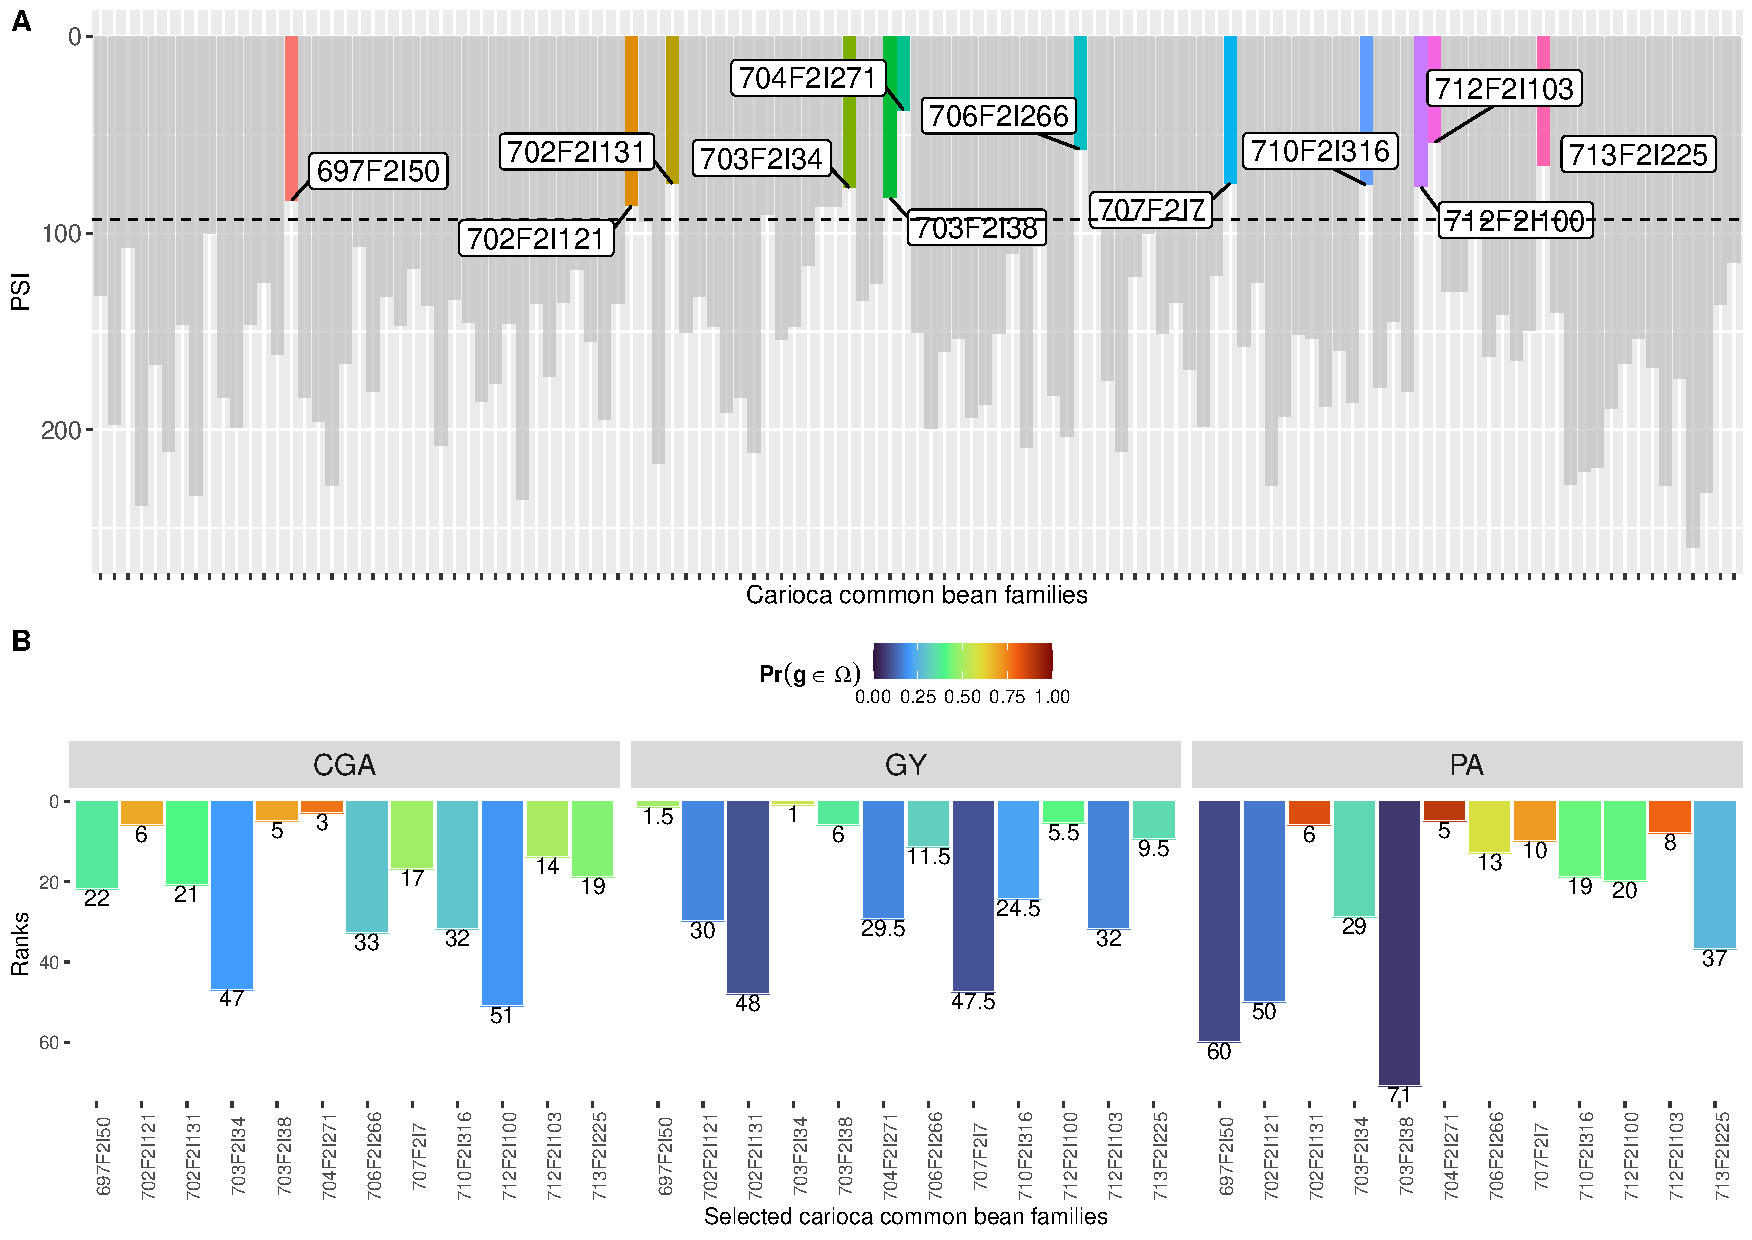
\includegraphics[width=0.6\linewidth,height=\textheight,keepaspectratio]{misc/images/PSIplot.pdf}

}

\caption{Probabilistic Selection Index visualization}

\end{figure}%
\end{frame}

\begin{frame}{Conclusion}
\phantomsection\label{conclusion}
Applying BPSI to carioca common bean panel, 12 families was selected
aiming to extract pure lines to GA, GY and PA simultaneously. BPSI has
potential to be applied on selection stage in breeding programs.
\end{frame}

\begin{frame}{Bibliography}
\phantomsection\label{bibliography}
\phantomsection\label{refs}
\begin{CSLReferences}{1}{0}
\bibitem[\citeproctext]{ref-Chagas2025}
Chagas, J. T. B., K. O. G Dias, V. Q. Carneiro, L. M. C. Oliveira, N. X.
Nunes, J. D. P. Júnior, P. C. S. Carneiro, and J. E. S. Carneiro. 2025.
{``Bayesian Probabilistic Selection Index in the Selection of Common
Bean Families.''} \emph{Crop Science} 65 (May): e70072.

\bibitem[\citeproctext]{ref-Dias2022}
Dias, K. O. G., J. P. R. dos Santos, M. D. Krause, H. P. Piepho, L. J.
M. Guimarães, M. M. Pastina, and A. A. F. Garcia. 2022.
{``\href{https://www.ncbi.nlm.nih.gov/pubmed/35192008}{Leveraging
Probability Concepts for Cultivar Recommendation in Multi-Environment
Trials}.''} \emph{Theoretical and Applied Genetics} 135 (April):
1385--99.

\bibitem[\citeproctext]{ref-Hazel1943}
Hazel, L N. 1943.
{``\href{https://www.ncbi.nlm.nih.gov/pubmed/17247099}{The Genetic Basis
for Constructing Selection Indexes.}''} \emph{Genetics} 28: 476--90.

\bibitem[\citeproctext]{ref-henderson1953estimation}
Henderson, Charles R. 1953. {``Estimation of Variance and Covariance
Components.''} \emph{Biometrics} 9 (2): 226--52.

\bibitem[\citeproctext]{ref-Kempthorne1959}
Kempthorne, Oscar, and Arne W Nordskog. 1959. {``Restricted Selection
Indices.''} \emph{Biometrics} 15: 10--19.

\bibitem[\citeproctext]{ref-Patterson1971}
Patterson, H D, and R Thompson. 1971. {``Recovery of Inter-Block
Information When Block Sizes Are Unequal.''} \emph{Biometrika} 58:
545--54. \url{https://doi.org/10.2307/2334389}.

\bibitem[\citeproctext]{ref-Peek1969}
Pešek, J., and R. J. Baker. 1969. {``DESIRED IMPROVEMENT IN RELATION TO
SELECTION INDICES.''} \emph{Canadian Journal of Plant Science} 49
(November): 803--4. \url{https://doi.org/10.4141/cjps69-137}.

\bibitem[\citeproctext]{ref-Smith1936}
Smith, H. F. 1936. {``A Discriminant Function for Plant Selection.''}
\emph{Annuals of Eugenics} 7: 240--50.

\end{CSLReferences}
\end{frame}




\end{document}
